% ----------------------------------------------------------------------
% ----------------------------------------------------------------------
%              Latex PhD template for the University of Deusto
% ----------------------------------------------------------------------


%: Style file for Latex
% Most style definitions are in the external file PhDthesisPSnPDF.
% In this template package, it can be found in ./Latex/Classes/
\documentclass[twoside,12pt]{Latex/Classes/PhDthesisPSnPDF}
\usepackage{enumitem, kantlipsum}
\usepackage{mathtools}
\usepackage{amssymb}
\usepackage[warn]{textcomp}
\usepackage{amsbsy}
\usepackage{pifont}
\usepackage{numprint}
\usepackage{lscape}
\usepackage{booktabs}
\usepackage{tikz}
\usepackage{notoccite}
\usepackage[export]{adjustbox}
\usepackage[ruled,vlined]{algorithm2e}
\usepackage{amsmath}
\usepackage{threeparttable, tablefootnote}
\usepackage{tabularx}
\usepackage[table]{xcolor}
\usepackage{array}

\DeclarePairedDelimiter\ceil{\lceil}{\rceil}
\DeclarePairedDelimiter\floor{\lfloor}{\rfloor}
\newcommand\scalemath[2]{\scalebox{#1}{\mbox{\ensuremath{\displaystyle #2}}}}
\newcommand{\cmark}{\ding{51}}
\newcommand{\xmark}{\ding{55}}
\newcommand{\ssep}{;}
\newcommand{\RFCOM}{\raisebox{2pt}{\tikz{\draw[-,black!40!black,solid,line width = 0.9pt](0,0) -- (5mm,0);}}}
\newcommand{\RFSM}{\raisebox{2pt}{\tikz{\draw[-,black!40!black,dashed,line width = 0.9pt](0,0) -- (5mm,0);}}}

\newcommand*\circled[1]{\tikz[baseline=(char.base)]{
            \node[shape=circle,draw,inner sep=1pt] (char) {#1};}}

\newcommand\diag[4]{%
  \multicolumn{1}{p{#2}|}{\hskip-\tabcolsep
  $\vcenter{\begin{tikzpicture}[baseline=0,anchor=south west,inner sep=#1]
  \path[use as bounding box] (0,0) rectangle (#2+2\tabcolsep,\baselineskip);
  \node[minimum width={#2+2\tabcolsep},minimum height=\baselineskip+\extrarowheight] (box) {};
  \draw (box.north west) -- (box.south east);
  \node[anchor=south west] at (box.south west) {#3};
  \node[anchor=north east] at (box.north east) {#4};
 \end{tikzpicture}}$\hskip-\tabcolsep}}


%: Macro file for Latex
% Macros help you summarise frequently repeated Latex commands.
% Here, they are placed in an external file /Latex/Macros/MacroFile1.tex
% An macro that you may use frequently is the figuremacro (see introduction.tex)
%---------------------------------------------------------------
% Macros
% version 3 by Igor Ruiz-Agundez 2011
% version 2 by Jakob Suckale 2007
% version 1 by Harish Bhanderi 2002
%---------------------------------------------------------------

% This file contains macros that can be called up from connected TeX files
% It helps to summarise repeated code, e.g. figure insertion (see below).



%---------------------------------------------------------------
% Figures
%---------------------------------------------------------------


% Makes the \InsertFig macro compatible both with one or two columns
\makeatletter
\newlength \figwidth
\if@twocolumn
  \setlength \figwidth {\columnwidth}
\else
  \setlength \figwidth {\textwidth}
\fi
\makeatother

% \InsertFig allows inserting figures
% Parameters
% 1 --> Filename
% 2 --> Label for referencing
% 3 --> Title describing the figure (caption)
% 4 --> Description of the figure
% 5 --> Figure width, range [0,1]. If parameter is left blank the figure size is not change
% 6 --> Any other option for \includegraphics
% Usage:
% \InsertFig{}{}{}{}{}{}
%
\newcommand{\InsertFig}[6]{%
	\ifthenelse{\isempty{#5}}%
	{% if #1 is empty
		\begin{figure}[htbp!]
		\centering
		\includegraphics[#6]{#1}%
		\caption{#3}{\textbf{#4}}
		\label{#2}
		\end{figure}    
	}
	{% if #1 is not empty
		% 20180625 LED: figuras preferentemente en top
		%\begin{figure}[htbp!]		
		\begin{figure}[!t]
		\centering
		\includegraphics[width=#5\figwidth,#6]{#1}%
		\caption{#3}{\textbf{#4}}
		\label{#2}
		\end{figure}
	}
}

%% Simple version of \InsertFig
%\newcommand{\InsertFig}[5]{
%  \begin{figure}[htbp]
%   	\centering
%    \includegraphics[width=#4\textwidth,#5]{#1}%
%    \caption{#3}
%    \label{#2}
%  \end{figure}
%}



% insert a centered figure with caption
% parameters 1:filename, 2:label, 3:title, 
\newcommand{\figuremacro}[3]{
	\begin{figure}[htbp]
		\centering
		\includegraphics[width=1\textwidth]{#1}
		\caption[#3]{\textbf{#3}}
		\label{#2}
	\end{figure}
}


% insert a centered figure with caption and description
% parameters 1:filename, 2:label, 3:title, 4:description
\newcommand{\figuremacroD}[4]{
	\begin{figure}[htbp]
		\centering
		\includegraphics[width=1\textwidth]{#1}
		\caption[#3]{\textbf{#3} - #4}
		\label{#2}
	\end{figure}
}

% insert a centered figure with caption and description AND WIDTH
% parameters 1:filename, 2:label, 3:title, 4:description, 5: textwidth
% textwidth 1 means as text, 0.5 means half the width of the text
\newcommand{\figuremacroDW}[5]{
	\begin{figure}[htbp]
		\centering
		\includegraphics[width=#5\textwidth]{#1}
		\caption[#3]{\textbf{#3} - #4}
		\label{#2}
	\end{figure}
}

% inserts a figure with wrapped around text; only suitable for NARROW figs
% o is for outside on a double paged document; others: l, r, i(inside)
% text and figure will each be half of the document width
% note: long captions often crash with adjacent content; take care
% in general: above 2 macro produce more reliable layout
\newcommand{\figuremacroN}[3]{
	\begin{wrapfigure}{o}{0.5\textwidth}
		\centering
		\includegraphics[width=0.48\textwidth]{#1}
		\caption[#2]{{\small\textbf{#2} - #3}}
		\label{#1}
	\end{wrapfigure}
}




% Estas definiciones son para el comando \InsertFigBox
\newlength{\anchoFigura}
\newlength{\anchoFloat}
\addtolength{\fboxsep}{2\fboxsep}
%\renewcommand{\capfont}{\normalfont\normalcolor\sffamily\small}
%\renewcommand{\caplabelfont}{\normalfont\normalcolor\sffamily\bfseries\small}

% El comando \InsertFigBox nos permite insertar figuras en un marco
% Los parametros son:
% 1 --> Fichero de la imagen
% 2 --> Etiqueta (label) para referencias
% 3 --> Texto a pie de imagen
% 4 -> Porcentaje del ancho de página que ocupará la figura (de 0 a 1)
% 5 --> Opciones que queramos pasarle al \includegraphics
\newcommand{\InsertFigBox}[5]{%
  \setlength{\anchoFloat}{#4\textwidth}%
  \addtolength{\anchoFloat}{-4\fboxsep}%
  \setlength{\anchoFigura}{\anchoFloat}%
  \begin{figure}%
    \begin{center}%
      \Ovalbox{%
        \begin{minipage}{\anchoFloat}%
          \begin{center}%
            \includegraphics[width=\anchoFigura,#5]{#1}%
            \caption{#3}%
            \label{#2}%
          \end{center}%
        \end{minipage}
      }%
    \end{center}%
  \end{figure}%
}



%---------------------------------------------------------------
% Misc
%---------------------------------------------------------------

% predefined commands by Harish
\newcommand{\PdfPsText}[2]{
  \ifpdf
     #1
  \else
     #2
  \fi
}


%---------------------------------------------------------------
% Locales
%---------------------------------------------------------------


%%
%% Para quitar traducciones raras (Cuadros)
%% A de usarse cada vez que se seleccione el idioma
%%
\newcommand{\MejorarTraducciones}{%
       \renewcommand{\listtablename}{Índice de tablas}
       \renewcommand{\tablename}{Tabla}
       \renewcommand{\lstlistingname}{Lista}
}%



%---------------------------------------------------------------
% Source code
%---------------------------------------------------------------


%%
%% Para escribir extractos de codigo
%%
%% Las tabulaciones se substituyen por dos espacios
%\fvset{tabsize=2}
%% Creamos un nuevo environment de fancyvrb para los ejemplos enmarcados
%\DefineVerbatimEnvironment{VerbEj}{BVerbatim}{fontsize=\small,samepage=true,commandchars=\\\{\}}
%% Colo de fondo
%\definecolor{grisfondo}{gray}{0.9}
%% Environment para extractos de codigo
%\newenvironment{codigo}%
%{\VerbatimEnvironment\begin{Sbox}\begin{VerbEj}}%
%{\end{VerbEj}\end{Sbox}\setlength{\fboxsep}{8pt}\begin{center}\fcolorbox{black}{grisfondo}{\TheSbox}\end{center}}
%
%% Otro formato más bonito para código fuente
%\newcommand{\codigofuente}[3]{%
%  \lstinputlisting[language=#1,caption={#2}]{#3}%
%}





%: ----------------------------------------------------------------------
%:                  TITLE PAGE: name, degree,..
% ----------------------------------------------------------------------
% 201803015 LED: I create some metadata to have a unique source for these fields
\def\myauthor{Ahmed Hamdy Madkour} % Author
%\def\mytitle{Pedestrian Localization using Wrist-Worn Smart Devices} % title
\def\mytitle{Learning in Non-stationary Envioronment } % title
\def\myadvisor{Dr. Amgad Monir and Prof. Hatem Mohamed} % Supervisor

% if output to PDF then put the following in PDF header
\ifpdf
    \pdfinfo { /Title  (\mytitle)
               /Creator (TeX)
               /Producer (pdfTeX)
               /Author (\myauthor)
               /CreationDate (D:201803150940)  %format D:YYYYMMDDhhmmss
               /ModDate (D:YYYYMMDDhhmm)
               /Subject (Pedestrian Localization)
               /Keywords (Auto machine learning, Concept drift, Imbalanced Stream, Transfer Learning, Emerging new Classes, and Dynamic Ensemble Selection.) }
    \pdfcatalog { /PageMode (/UseOutlines)
                  /OpenAction (fitbh)  }
    % 201803015 LED: \pdfinfo does not work in combination with hyperref
    \hypersetup{
    	pdfinfo={
    			Title={\mytitle},
                Author={\myauthor},
                Creator={TeX},
                Producer={pdfTeX},
                CreationDate={D:201803150940},
                ModDate={D:\pdfdate},
                Subject={Transportation},
                Keywords={Auto machine learning, Concept drift, Imbalanced Stream, Transfer Learning, Emerging new Classes, and Dynamic Ensemble Selection.}
    	}
}
\fi


% ----------------------------------------------------------------------

% turn of those nasty overfull and underfull hboxes
\hbadness=10000
\hfuzz=50pt



\begin{document}

%\selectlanguage{british}
\selectlanguage{english}

% sets line spacing
\renewcommand\baselinestretch{1.2}
\baselineskip=18pt plus1pt

% As abstract contains various languages we set the main language again
%\selectlanguage{british}
\selectlanguage{english}


%: ----------------------- contents ------------------------

\setcounter{secnumdepth}{5} % organisational level that receives a numbers
\setcounter{tocdepth}{5}    % print table of contents for level 3


%%You can also add extra lines to the ToC or to force extra unnumbered section headings to be included. For example, if you wanted to add an entry called Preface, and you didn't want the Preface to be numbered, you'd use these commands:
%\ subsection*{Preface}
%\addcontentsline{toc}{subsection}{Preface}

% \tableofcontents            % print the table of contents
% % levels are: 0 - chapter, 1 - section, 2 - subsection, 3 - subsection

% %: ----------------------- list of figures/tables ------------------------

%: ----------------------- glossary ------------------------
% 20180315 LED: for WinEdt it is necessary to install the Nomenclature.zip that is available in the WindEdt website

% Tie in external source file for definitions: /0_frontmatter/glossary.tex
% Glossary entries can also be defined in the main text. See glossary.tex

%\begin{multicols}{2} % \begin{multicols}{#columns}[header text][space]
%\begin{footnotesize} % scriptsize(7) < footnotesize(8) < small (9) < normal (10)

% Parts of the thesis are included below. Rename the files as required.
% But take care that the paths match. You can also change the order of appearance by moving the include commands.

% 20180315 LED:
%\include consideres the file as a section, introducing a page break after it and placing all the figures inside that section;
%\input only concatenates the content of the files, without assuming anything else

%: ----------------------- introduction ------------------------
%\part{Proposal}
% introduction

% this file is called up by thesis.tex
% content in this file will be fed into the main document


% this file is called up by thesis.tex
% content in this file will be fed into the main document

%: ----------------------- introduction file header -----------------------


\begin{savequote}[50mm]
Success is the sum of small efforts, repeated day-in and day-out.
\qauthor{Robert Collier}
\end{savequote}

\chapter{Introduction}
\label{cha:1_Introduction}

% the code below specifies where the figures are stored
\ifpdf
    \graphicspath{{1_introduction/figures/PNG/}{1_introduction/figures/PDF/}{1_introduction/figures/}}
\else
    \graphicspath{{1_introduction/figures/EPS/}{1_introduction/figures/}}
\fi


%-------------------------------------------------------------------------
%Chapter 1 contents:
%- Motivation of the research field: Context-aware systems -> LBS -> GNSS limitation -> Positioning techniques -> DR -> inertial PDR -> inertial PDR + wearables
%- Problem identification: smartphone not a wearable -> potentiality of wrist-worn wearables -> Problem: no wrist-worn PDRS
%- Goal of the thesis: tackle the problem -> how? Splitting it into sub-problems
%- Structure of the thesis
%-------------------------------------------------------------------------

Governments and companies are producing vast streams of data and require effective data analytics and machine learning methods to assist in making predictions and decisions promptly. One crucial aspect is the machine learning pipeline, which involves training a prepared dataset to construct a model and subsequently utilizing this model to predict new instance outputs. As depicted in Fig. \ref{fig:machine-old-senario}, the process entails fetching historical data from the database during the training phase to construct the machine learning model. Then, the system can input new instances from the database to predict the output.

\begin{figure}[!ht]
    \centering
    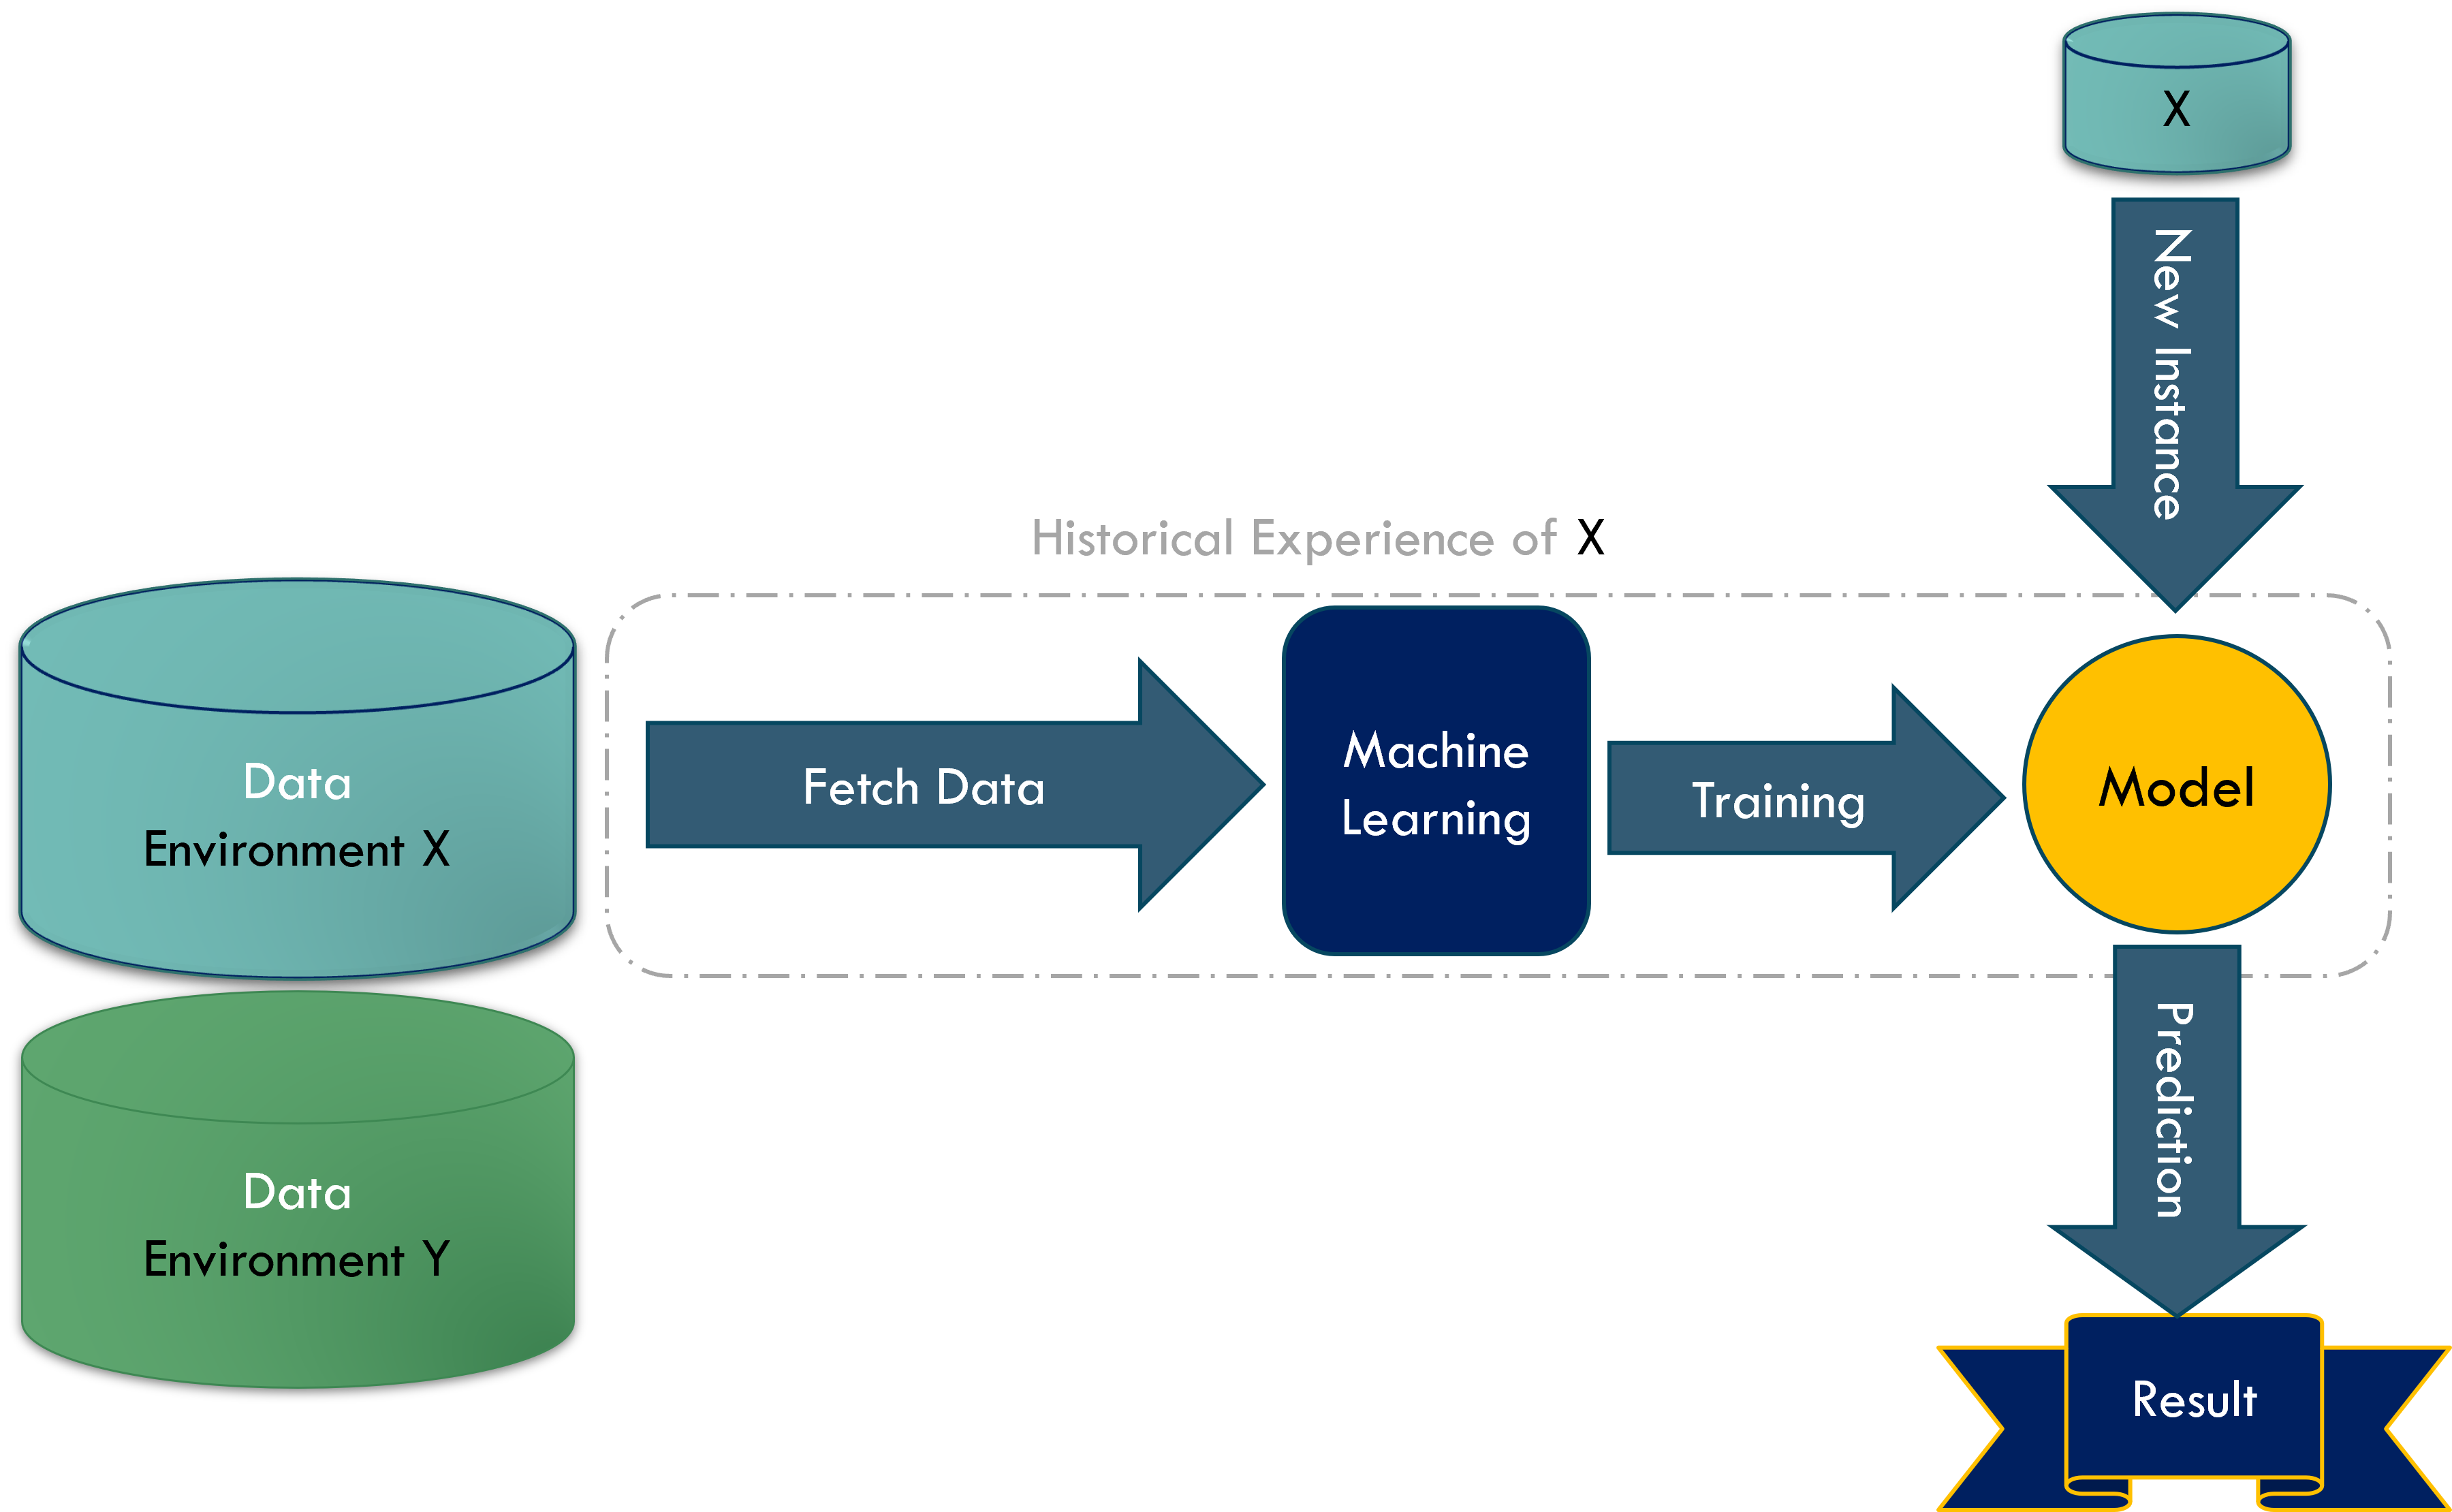
\includegraphics[width=.9\textwidth]{1_introduction/figures/PNG/machine_flow.png}
    \caption{The research methodology of the thesis.}
    \label{fig:machine-old-senario}
\end{figure}

Nevertheless, when endeavoring to forecast outcomes for fresh instances sourced from an alternative database, as illustrated in Fig. \ref{fig:machine-new-senario}
, there frequently emerges a conspicuous decline in accuracy. This disparity accentuates the imperative for model developers to intervene and rectify the issue. Addressing this, developers must adjust and retrain the model utilizing datasets from the new environment to ameliorate accuracy. This iterative process aims to refine the model's precision and ensure its efficacy across diverse contexts, thereby bolstering the reliability of decision-making and predictive capabilities. To confront this challenge, the field of auto machine learning endeavors to facilitate online updates to the model without necessitating direct intervention from developers for modification.

\begin{figure}[!ht]
    \centering
    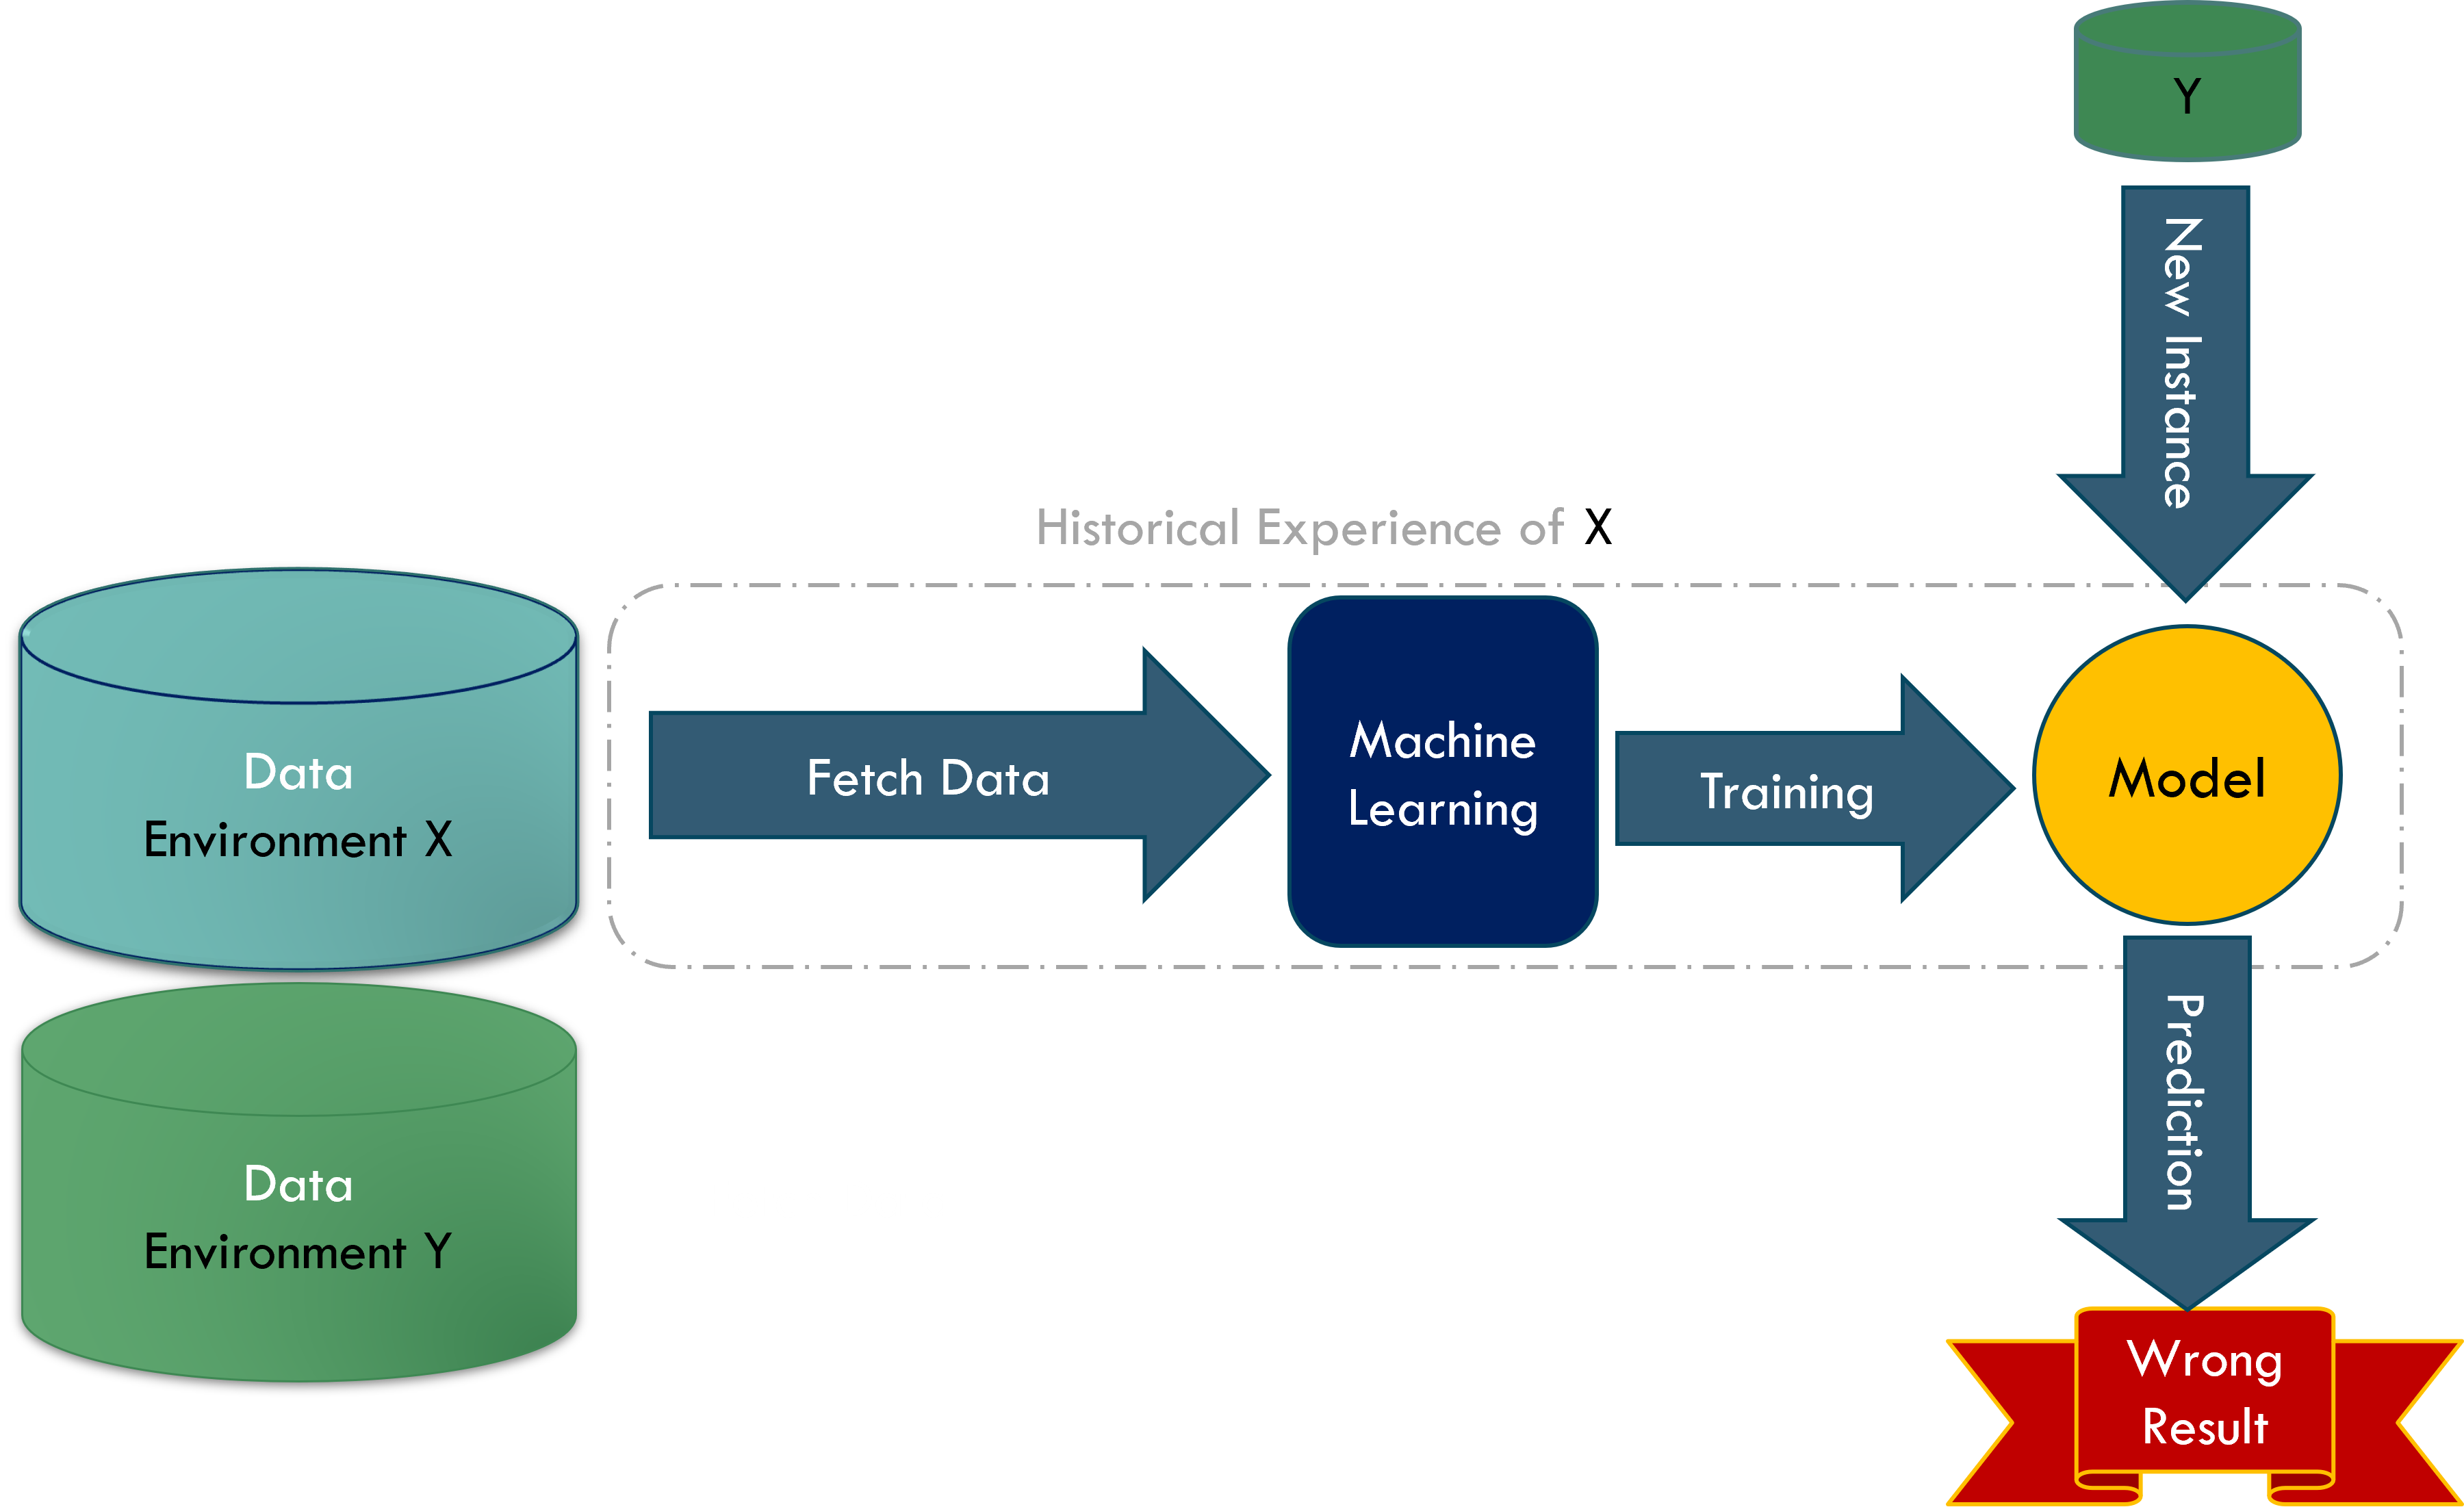
\includegraphics[width=.8\textwidth]{1_introduction/figures/PNG/wrong_machine_flow_1.png}\\
    (a) \\
    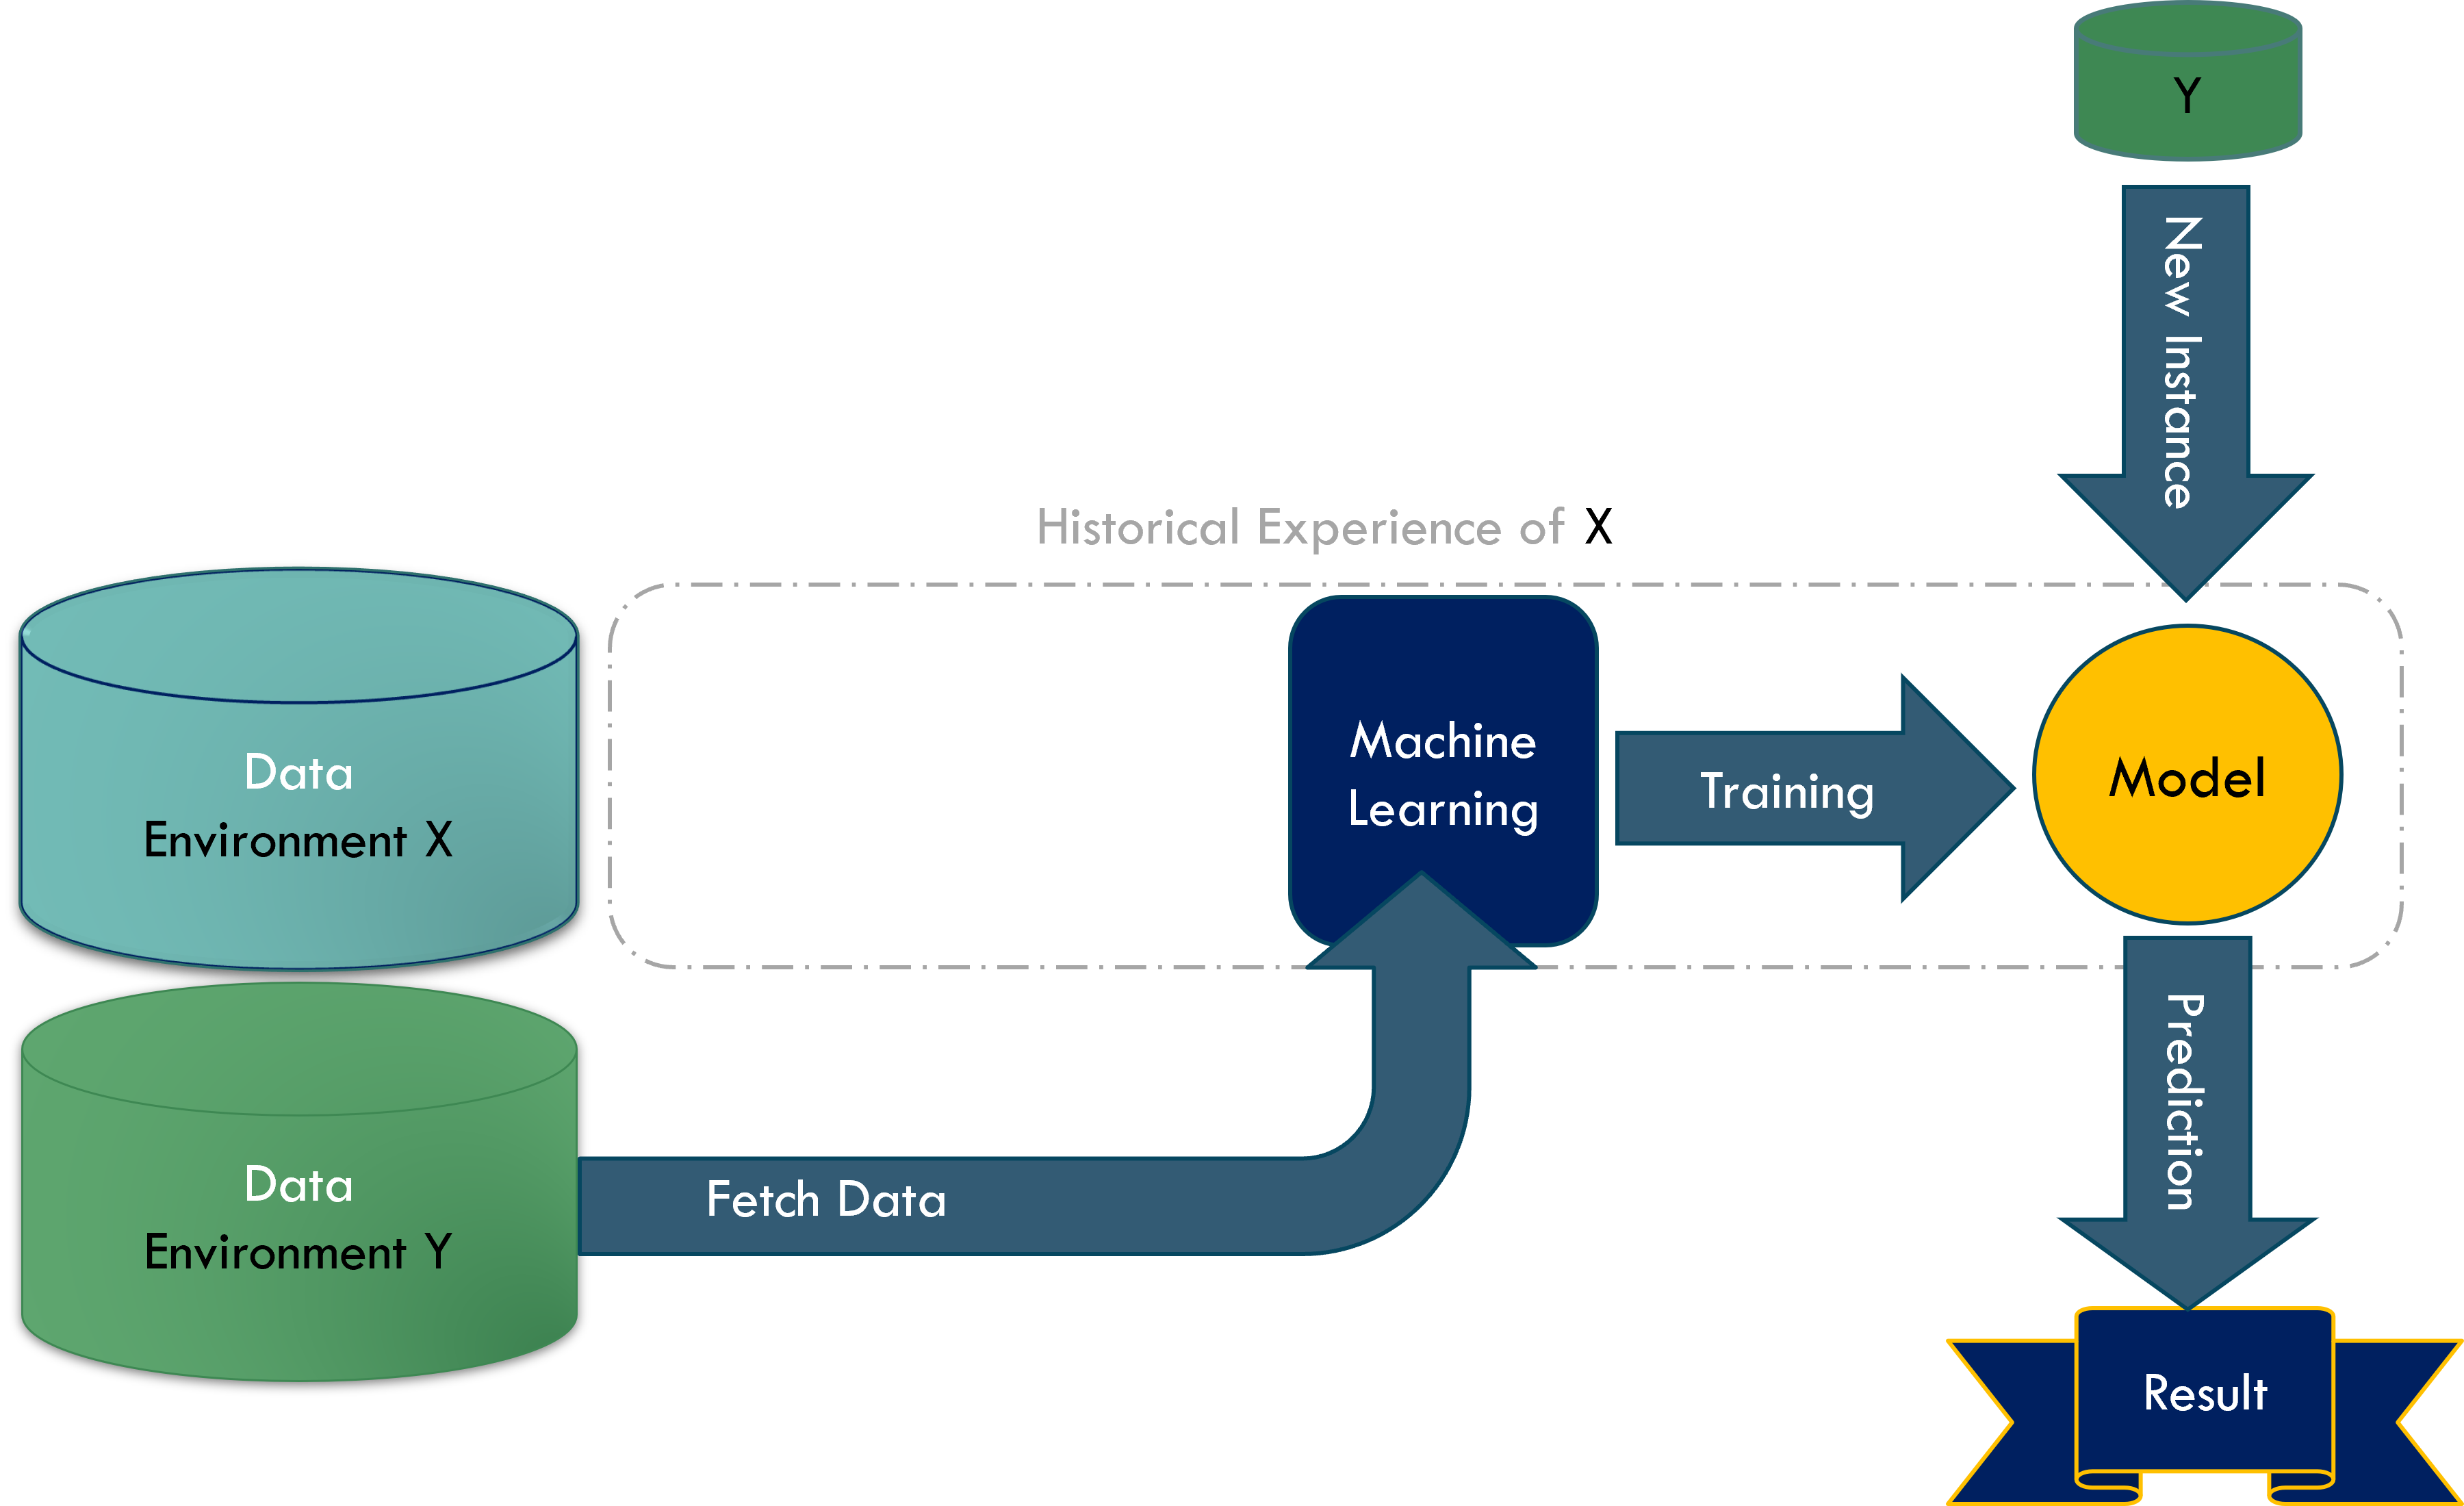
\includegraphics[width=.8\textwidth]{1_introduction/figures/PNG/wrong_machine_flow_2.png}\\
    (b)
    \caption{The research methodology of the thesis.}
    \label{fig:machine-new-senario}
\end{figure}



In recent years, the surge in high-speed data streams has posed notable challenges for machine learning models, particularly in the context of streaming data analysis. These data streams, characterized by continuous, dynamic, and high-volume data arrivals, demand adaptive learning algorithms that can effectively cope with their evolving nature \cite{yang2021concept} \cite{dong2019multistream} \cite{shan2018online}. Within these evolving data environments, two paramount challenges have emerged: concept drift, class imbalance, Emerging new class, and heterogenous transfer learning.

Concept drift, a phenomenon defined by the evolving statistical properties of a data generation process over time \cite{pan2009survey} \cite{zhuang2020comprehensive}. introduces a dynamic element to the data, necessitating continuous adaptation of machine learning models. This shift can manifest as changes in underlying concepts, relationships between variables, or alterations in data distribution. Traditional models trained on historical data may suffer diminished accuracy or become inadequate when confronted with new data influenced by concept drift, highlighting the need for effective concept drift detection mechanisms. Addressing concept drift involves the utilization of concept drift detectors, which are methods capable of identifying changes in data stream distributions. These detectors rely on information related to classifier performance or incoming data items to signal the need for model updates, retraining, or even replacing the old model with a new one. The dynamic nature of concept drift necessitates ongoing monitoring and adaptation to maintain the model's efficacy.

Data streams also present challenges related to class imbalance, a condition characterized by uneven distribution among different classes \cite{wang2018systematic} \cite{sun2009classification}. This scenario, especially prevalent in multi-class settings, poses a significant challenge for traditional classifiers. The risk of misclassifying minority class samples due to their limited representation demands specialized techniques to ensure accurate classification without sacrificing the performance of the majority class \cite{charte2015addressing} \cite{charte2015mlsmote} \cite{daniels2017addressing} \cite{liu2018making}. To tackle class imbalance, three primary methods are commonly employed: sampling methods, algorithm adaptation methods, and hybrid methods. Sampling methods involve undersampling the majority class or oversampling the minority class to balance class distribution. Algorithm adaptation methods modify existing algorithms to handle imbalanced data \cite{japkowicz1995novelty} \cite{lopez2012analysis} \cite{zhang2020towards}, while hybrid methods combine data preprocessing with classification techniques, often utilizing ensemble classifiers to effectively mitigate class imbalance and enhance overall classifier performance \cite{chawla2003smoteboost} \cite{wang2010negative} \cite{galar2011review} \cite{cruz2018dynamic}.

Another challenge arising in the context of class imbalance is class overlap, where instances from different classes share the same region in data space \cite{bhowan2012evolving} \cite{galar2011review}. This overlap complicates the task of distinguishing between representative instances of different classes, leading to performance challenges for traditional classifiers referred to as overlapping problems. Recent research introduces class-overlap undersampling methods to address this issue, leveraging local similarities among minority instances to identify potentially overlapping majority instances.

Therefore, both class imbalance and class overlap present significant hurdles in the realm of data stream analysis. Consequently, addressing class imbalance has become crucial in multi-class learning, leading to research efforts focusing on both concept drift and class imbalance challenges. Researchers have explored dynamic ensemble selection (DES) and multi-class oversampling techniques to tackle these issues. Dynamic classifier ensembles offer a unique ability to adapt their composition based on data characteristics, making them valuable in situations with evolving data conditions \cite{cruz2018dynamic}. Researchers focus on the overproduce-and-select approach for classifier ensemble selection methods. The objective of classifier ensemble selection is to choose an optimal subset of classifiers from a larger ensemble. The selection process is guided by various criteria, including individual performance measures, diversity metrics, meta-learning techniques, and performance estimation approaches. This optimization is particularly important in scenarios where a balance between accuracy and computational resource constraints is critical. There are two distinct approaches: static and dynamic selection. Static selection involves assigning classifiers to predefined feature partitions, while dynamic selection adaptively selects classifiers based on their competency \cite{kuncheva2000clustering}. Dynamic selection offers two choices: individual models, known as Dynamic Classifier Selection (DCS), and ensemble models, called Dynamic Ensemble Selection (DES). DCS algorithms enable the selection of the most appropriate classifier for each data point based on its local competencies. In contrast, DES focuses on selecting the optimal classifiers for each instance based on their competence within localized regions \cite{woloszynski2011probabilistic} \cite{lysiak2014optimal} \cite{cruz2017meta} Competency assessment relies on a dynamic selection dataset (DSEL) containing labeled samples. Moreover, innovative techniques like the Randomized Reference Classifier introduce randomness into class supports to enhance adaptability in addressing challenges related to imbalanced data.

Additionally, transfer learning assumes a pivotal role in addressing the intricate challenges posed by dynamic data streams and inherent concept drift. This domain of research focuses on enhancing a model's learning performance within a target domain by harnessing knowledge gleaned from source domains \cite{pan2009survey} \cite{wang2018systematic}.Techniques in transfer learning include reducing domain gaps through instance re-weighting and feature matching, along with strategies to mitigate negative knowledge transfer by down-weighting irrelevant source data.

Lastly, in the study, the focus extends to the specific scenario of Streams with Emerging New Classes (SENC). This refers to situations where new classes, not present during the initial training of a learning model, emerge in the data stream. Traditional learning approaches, designed for fixed or predefined class distributions, face challenges in effectively recognizing and adapting to these novel classes in real-time. The need for adaptive learning mechanisms that can handle the emergence of new classes underscores the complexity of real-world data stream scenarios.
     

In this chapter, the challages for this research 
that naturally arise is discussed in  Section \ref{sec:1_introduction_challange}. After this, the the motivation, scope and solution methodology are presented in Section \ref{sec:1_introduction_motivation} . After this, the objectives and
esearch questions are presented in Sections \ref{sec:1_introduction_objectives} and \ref{sec:1_introduction_questions}, respectively. Next, the
research contribution is summarised in Section \ref{sec:1_3_automl_and_tf}. Next the research publication is presented in Section \ref{sec:1_introduction_publication}. Finally,
the research methodology and the outline of this thesis are presented in Sections \ref{sec:1_introduction_methodology} and
\ref{sec:1_introduction_organizations}, respectively.
\section{Challenges}
\label{sec:1_introduction_challange}
Within the swiftly evolving realm of machine learning, the proliferation of high-speed data streams presents a significant hurdle — the proficient management of non-stationary data environments. This challenge is marked by dynamic fluctuations in statistical attributes, fundamental concepts, and data distributions over time. The crux of the issue emerges as models, initially trained on historical data, experience a decline in accuracy when confronted with new data influenced by concept drift. This includes scenarios such as:
\begin{itemize}
    \setlength{\itemsep}{0pt}
    \setlength{\parskip}{0pt}
    \item Multi-class imbalanced data streams
    \item Overlapping classes
    \item Emergence of new classes
    \item Heterogeneous transfer learning
\end{itemize}
However, addressing these challenges yields substantial benefits. By effectively managing non-stationary data environments, organizations can enhance the adaptability and resilience of their machine learning systems. This enables more robust decision-making processes, improved predictive capabilities, and heightened performance across diverse contexts. Moreover, it fosters innovation and agility, empowering organizations to stay ahead in dynamic markets and evolving scenarios.

\section{Thesis Motivations}
\label{sec:1_introduction_motivation}

The swift progress in machine learning, particularly in real-time data streams, introduces new challenges that demand innovative solutions. This thesis seeks to address the limitations of traditional models in dynamic, non-stationary data environments. The motivations behind this research are as follows:
\begin{itemize}
    \setlength{\itemsep}{0pt}
    \setlength{\parskip}{0pt}
    \item \textbf{Adapting to Emerging Classes in Real-Time:} New classes within data streams can cause a decline in accuracy. The goal is to develop adaptive mechanisms that quickly incorporate new classes, maintaining system relevance.
    \item \textbf{Proactive Management of Concept Drift:} Concept drift degrades model performance as data properties change. This research focuses on strategies to detect and manage concept drift to maintain model accuracy.
    \item \textbf{Dynamic Optimization of Classifier Ensembles:} To handle emerging classes and shifting distributions, we aim to develop techniques for real-time optimization of classifier ensembles.
    \item \textbf{Addressing Multi-Class Imbalance:} Imbalanced multi-class distributions often lead to biased classification. The thesis aims to create methods that address class imbalances dynamically, ensuring fair classification.
    \item \textbf{Enhancing Transfer Learning in Non-Stationary Environments:} Transfer learning can suffer from negative transfer in non-stationary settings. The research focuses on frameworks that minimize negative transfer and enhance knowledge sharing across diverse domains.
\end{itemize}

\section{Thesis Objectives}
\label{sec:1_introduction_motivation}
The thesis objectives for our research stems from the imperative need to address the following key motivations:
\begin{itemize}
    \item \textbf{Objective 1}. Thandling Imbalanced Multiclass Drifted Data and overlapping classes streams.
    \item \textbf{Objective 2}. addressing Emerging New Classes in Incremental Streams via Concept Drift and K-means Techniques.
    \item \textbf{Objective 3}. addressing Heterogeneous Transfer Learning Problem in data streams via Concept Drift and Eigenvector Techniques.
\end{itemize}

\section{Thesis Questions}
\label{sec:1_introduction_questions}

\begin{itemize}[nosep]
    \setlength{\itemindent}{-.5in}
       \item $\pmb{Q_1}$. What is the impact of imbalanced stream on the performance of ML models in Nonstationary Environment?
        \item $\pmb{Q_2}$. What is the impact of reducing overlapping classes stream on the performance of ML models in Nonstationary Environment?
        \item $\pmb{Q_3}$.How does the emergence of new classes in data streams affect the stability and performance of ML models?
        \item $\pmb{Q_4}$. how can ML models be adapted to accommodate such changes?
        \item $\pmb{Q_5}$. how to employee concept drift to solve the emerging new classes problem?
        \item $\pmb{Q_6}$. How does the Heterogeneous sources in data streams affect the stability and performance of Transfer Learning Technique?
        \item $\pmb{Q_7}$. What approaches or techniques can be employed in heterogeneous transfer learning to facilitate knowledge transfer across diverse sources and domains?
    \end{itemize}
    
\section{Contributions}
\label{sec:1_introduction_contribution}
Our research endeavors to create advanced frameworks designed for effectively managing non-stationary data streams while prioritizing high accuracy and minimizing computational complexity. The key contributions of our work can be summarized as follows:
\begin{itemize}
    \item \textbf{Incorporation of Concept Drift Detection and Ensemble Classifier:} Our primary innovation involves incorporating a concept drift detection method alongside an ensemble classifier. This integration enables real-time adaptation and refinement of our proposed framework in response to transfer learning in non-stationary environments. This methodology ensures the continuous evolution of our classification model in alignment with the changing data landscape.
    \item \textbf{Dynamic Classifier Ensemble Framework for Emergence Class Problem:} We introduce a classification framework that harnesses dynamic classifier ensemble techniques to address the emergence class problem. This framework enhances the performance of classification algorithms when dealing with non-stationary data streams featuring emerging new classes. By dynamically adjusting the ensemble based on data characteristics, our framework improves the accuracy and effectiveness of classification models, effectively tackling challenges associated with emerging new classes.
    \item \textbf{Introduction of Precise Weighting Method for Local Classifiers of the transfer learning framework:} A significant advancement in our research is the introduction of a precise weighting method to assess the significance of each local classifier within the ultimate classifier. This method enhances the accuracy of the overall classifier by providing a nuanced evaluation of individual classifier contributions.
    \item \textbf{Development of Innovative Framework using Eigenvector Technique for addressing heterogenous transfer learning problem:} A significant stride in our research involves the creation of an innovative framework, harnessing the power of the eigenvector technique. This framework is specifically designed to tackle the challenges posed by heterogeneous transfer learning problems. By leveraging the eigenvector technique, our framework enables the seamless transfer of knowledge from diverse source domains to the target domain, thereby enhancing adaptability and overall performance.
    \item \textbf{Dynamic Adjustment Method to Multi-class Imbalanced Data:} Our classification framework introduces a dynamic adjustment method tailored for multi-class imbalanced data scenarios. It seamlessly incorporates concept drift detection mechanisms and optimizes classifier ensemble selections, aiming to significantly improve classification accuracy in the context of multi-class imbalanced non-stationary streams.
    \item \textbf{Adaptive Method for Class Imbalance:} Additionally, we propose an adaptive method for addressing the class imbalance issue. This method considers data distributions and historical instances of class imbalance, especially in cases where class overlap occurs within multi-class and drifted data streams. The adaptive approach improves classification performance by selecting the most suitable oversampling method based on the unique characteristics of the data stream.
\end{itemize}


\section{Publications}
\label{sec:1_introduction_publication}
\begin{table}[h]
 \centering
 \resizebox{\textwidth}{!}{
\renewcommand{\arraystretch}{1.1}
\begin{tabular}{l}
\hline
\textbf{Title:} Dynamic Classification Ensembles for Handling Imbalanced Multiclass Drifted Data Streams.\\
\textbf{Authors:} Madkour, Ahmed H.,Hatem M. Abdelkader, and Amgad M. Mohammed\\
 \textbf{Journal:} Information systems (Impact Factor $=$ 8,1 $\rightarrow$ Q1).\\
 \textbf{Status:} Published. \\ \hline

 \textbf{Title:} Historical Isolated Forest for detecting and adaptation concept drifts in non-stationary data streaming.\\
 \textbf{Authors:} Madkour, Ahmed H.,Hatem M. Abdelkader, and Amgad M. Mohammed.\\
 \textbf{Journal:}  IJCI. International Journal of Computers and Information, 10.2 2023. \\ \textbf{Status:} Published.\\ \hline

\textbf{Title:} Addressing Emerging New Classes in Incremental Streams via Concept Drift Techniques.\\
 \textbf{Authors:} Ahmed H., Madkour, Enrique Onieva, Hatem M. Abdelkader, and Amgad M. Mohammed.\\
 \textbf{Journal:} Information Systems (Impact Factor $=$ 3,0 $\rightarrow$ Q1).\\
 \textbf{Status:} Under review. \\ \hline
 


 
\textbf{Title:} Addressing Heterogeneous Transfer Learning Problem in data streams via Concept Drift.\\
\textbf{Authors:} Ahmed H., Madkour, Enrique Onieva, Hatem M. Abdelkader, and Amgad M. Mohammed.\\
 \textbf{Journal:} Evolving Systems (Impact Factor $=$ 2.8 $\rightarrow$ Q2).\\
 \textbf{Status:} Under review. \\ \hline
 
 
\end{tabular}
 }
 \caption{Publications in journals and conferences conducted during this thesis.}
\label{ch1.publication.list}
\end{table}
During the research activities of this thesis, several international peer-reviewed
journal articles were published to disseminate the obtained results. The publications can be found in Table \ref{ch1.publication.list}. 

\section{Thesis Plan}
\label{sec:1_introduction_methodology}
\begin{figure}[!ht]
    \centering
    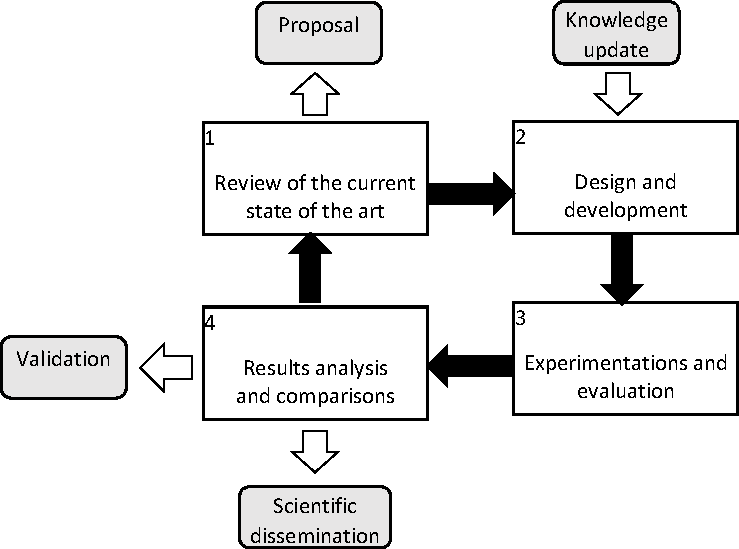
\includegraphics[width=.8\textwidth]{1_introduction/figures/fig_research-methodo.pdf}
    \caption{The Research Plan of Thesis.}
    \label{ch1:research-emthodo}
\end{figure}

The research in this thesis is progressing rapidly due to technological advancements and continuous contributions in machine learning (ML). An iterative research methodology was followed, where each cycle builds upon the knowledge gained in the previous phase, leading to increasingly effective and original solutions as shown in Fig. \ref{ch1:research-emthodo}. The phases of this research methodology are as follows:

\begin{enumerate}
    \setlength{\itemsep}{0pt}
    \setlength{\parskip}{0pt}
    \item \textbf{Review of the current state-of-the-art:} Investigate existing research to identify challenges and inform the design of a solution.
    \item \textbf{Design and development:} Design a novel solution using updated knowledge to address the identified challenges.
    \item \textbf{Experimentation and evaluation:} Test the solution through experimentation, using established criteria for comparison.
    \item \textbf{Results analysis and comparison:} Analyze and compare results with state-of-the-art to determine the effectiveness of the solution, and disseminate the findings.
\end{enumerate}



\section{Structure of the Dissertation}
\label{sec:1_introduction_organizations}
The structure of the remainder of this thesis dissertation is outlined below.
\begin{itemize}	
	\item \textbf{Chapter~\ref{cha:2_background}} reviews background about concept drift, concept drift types, concept drift components, adapting types.  
	
	\item \textbf{Chapter~\ref{cha:3_State-of-the-art}} reviews state-of-the-art  concept drift, classifier ensemble selection, imbalanced data streams, Streams with Emerging New Classes (SENC), and transfer learning.  
	
	\item \textbf{Chapter~\ref{chapter:4_Imbalanced_Multiclass}
	} presents our first proposal to build an effective proposed approch for  handling Imbalanced Multi-class Drifted Data streams.
	
	\item \textbf{Chapter~\ref{chapter:5_emerging}} provides our second proposal to adressing emerging new classes in incremental streams via concept drift techniques. 
	
	\item \textbf{Chapter~\ref{chapter:6_transfer_learning}} presents our third proposal to addressing heterogeneous transfer learning problem  in incremental streams via concept drift techniques.
	
	\item \textbf{Chapter~\ref{chapter:7_Conclusions}} revisits the main goal and specific objectives posted earlier. In this chapter, we summarise the main contributions of this thesis and outline possible future research.


\end{itemize}

% background
% this file is called up by thesis.tex
% content in this file will be fed into the main document


\chapter{Background}\label{cha:2_background}

Amidst the surge of vast streaming data, governments and businesses find themselves in an urgent need for sophisticated data analysis and machine learning analytics approaches. These tools are indispensable for anticipating future trends and making well-informed decisions. However, the perpetual emergence of new goods, markets, and consumer behaviors introduces a formidable challenge known as concept drift \cite{widmer1996learning}. This phenomenon involves the variation of statistical parameters of the target variable over time in unexpected ways, posing a substantial obstacle to accurate forecasting and optimal decision-making. The patterns derived from historical data may become obsolete when applied to new and evolving datasets.
The impact of concept drift extends across data-driven information systems, including decision support and early warning systems, diminishing their overall effectiveness. In the dynamic realm of big data, where data types and distributions are inherently unpredictable, the challenge of concept drift becomes even more pronounced. In response to this challenge, the field introduces a new subject: adaptive data-driven prediction/decision systems.

\section{Concept Drift Sources}
\vspace{-3mm}
\begin{figure}[H]
    \centering
    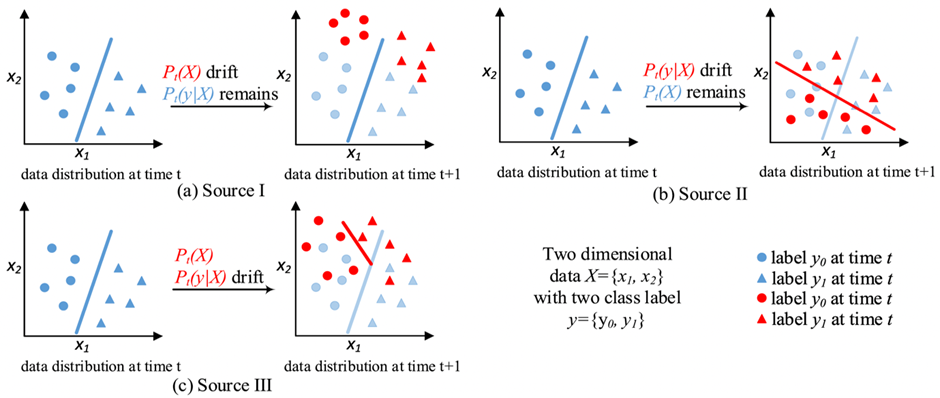
\includegraphics[width=1.0\textwidth]{2_Background/figures/concept_drift_sources.png}
    \caption{Sources of Concept Drift \cite{8496795}. \\ \textcolor{gray}{\fontsize{10}{0}\selectfont DOI: 10.1109/TKDE.2018.2876857}}
    \label{fig:concept-drift-sources}
\end{figure}
\vspace{-6mm}
\label{sec:background_concept_drift_sources}
Concept drift, as illustrated in Fig. \ref{fig:concept-drift-sources}, occurs in three distinct scenarios. First, (a) depicts a shift in data distribution, indicating changes in the underlying patterns and characteristics of incoming data, challenging the model's ability to adapt to new trends \cite{lu2016concept, gama2014survey, losing2016knn, storkey2008training}. Second, (b) shows a change in function output, requiring adjustments in the class delimiter's position as the relationship between input features and output classes evolves. Lastly, (c) represents a dual shift in both data distribution and function output, a more complex form of concept drift that requires the model to adapt to simultaneous changes in patterns and output relationships. Effectively managing these shifts is essential for maintaining predictive accuracy and decision-making in dynamic environments, highlighting the importance of adaptive strategies in machine learning models.



\section{Concept Drift Types}
\label{sec:background_concept_drift_types}
Concept drift is categorized into four types, as shown in Fig. \ref{fig:concept-drift-types}. Types 1-3 focus on minimizing accuracy loss and maximizing recovery during concept transformation. Type 4, however, emphasizes leveraging historical concepts to identify the best-matched concept during new concept emergence. The term "intermediate concept," introduced by \cite{losing2016knn}, refers to transitional phases between concepts. \cite{liu2018making} further notes that concept drift can extend over time, with intermediate concepts representing a blend of starting and ending concepts in incremental drift or one of these in gradual drift. Understanding these intermediate concepts is key to grasping the dynamics of concept drift during transitions.
\vspace{-3mm}
\begin{figure}[H]
    \centering
    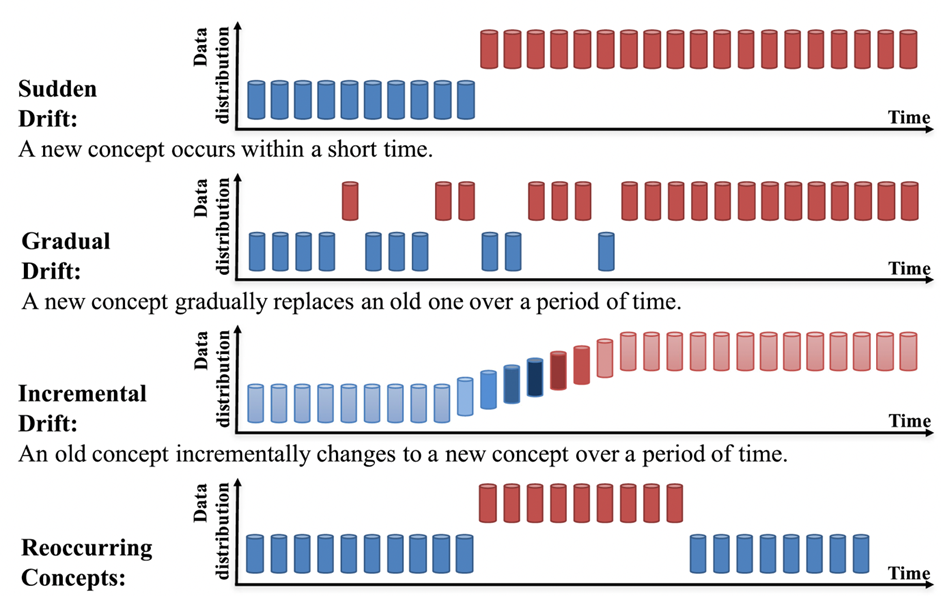
\includegraphics[width=0.8\textwidth]{2_Background/figures/concept_drift_types.png}
    \caption{Types of Concept Drift \cite{8496795}. \\ \textcolor{gray}{\fontsize{10}{0}\selectfont DOI: 10.1109/TKDE.2018.2876857}}
    \label{fig:concept-drift-types}
\end{figure}
\vspace{-6mm}


\section{Concept Drift Components}
\label{sec:background_concept_drift_components}
Conventional machine learning primarily involves prediction and training/learning. However, learning under the concept drift paradigm introduces three additional critical steps as show in Fig. \ref{fig:concept-drift-components}: concept drift detection, drift understanding, and drift adaptation. Concept drift detection involves identifying changed points or change time periods to define and predict drift. Drift understanding delves into crucial aspects such as when the drift starts, how long it lasts, and where it occurs, providing indispensable insights for the subsequent adaptation step.  
The adaptation step, also referred to as the reaction step, plays a pivotal role in updating current learning models in response to concept drift. Three main approaches address various types of drift: Simple Retraining, Ensemble Retraining, and Model Adjusting. Drift detection employs various tools and algorithms, comparing old and fresh data chunks with statistical models based on data distribution. Techniques vary, with some utilizing a constant chunk length and others employing a variable length.
Drift understanding is essential for making well-informed decisions during the adaptation step. This involves calculating the necessary modifications in the trained model to adapt to new changes as shown in Fig. \ref{fig:concept-drift-understanding}. The severity region determines whether to generate a completely new model or make minimal adjustments to the existing one.

 
\begin{figure}[!ht]
    \centering
    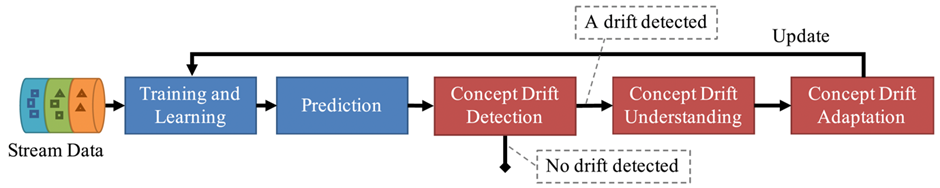
\includegraphics[width=.9\textwidth]{2_Background/figures/concept_drift_components.png}
    \caption{Main components of concept drift. \\ \textcolor{gray}{\fontsize{10}{0}\selectfont DOI: 10.1109/TKDE.2018.2876857}}

    \label{fig:concept-drift-components}
\end{figure}


%==============================[detection subsection]===============
\subsection{Concept Drift Detection}
Drift detection involves techniques and mechanisms to characterize and quantify concept drift by identifying change points or intervals \cite{liu2018making}. The general framework for drift detection consists of four stages:
\begin{itemize}
    \item \textbf{Stage 1 (Data Retrieval):} This stage focuses on retrieving data chunks from data streams. Given that a single data instance lacks sufficient information to infer the overall distribution \cite{lu2016concept}, organizing data chunks meaningfully is crucial for effective data stream analysis \cite{ramirez2017survey}.
    \item \textbf{Stage 2 (Data Modeling):} This optional stage abstracts the retrieved data, extracting key features that contain sensitive information impacting a system in case of drift. This stage may involve dimensionality reduction or sample size reduction to meet storage and online speed requirements \cite{liu2018making}.
    \item \textbf{Stage 3 (Test Statistics Calculation):} This stage involves measuring dissimilarity or estimating distance to quantify drift severity and generate test statistics for hypothesis testing. Defining an accurate and robust dissimilarity measurement remains a challenging aspect of concept drift detection. Test statistics can also be used for clustering evaluation \cite{silva2013data} and to determine dissimilarity between sample sets \cite{dries2009adaptive}.
    \item \textbf{Stage 4 (Hypothesis Test):} This stage employs a specific hypothesis test to assess the statistical significance of the change observed in Stage 3, such as the p-value. These tests determine drift detection accuracy by establishing statistical bounds for the test statistics from Stage 3. Without Stage 4, the acquired test statistics are meaningless for drift detection, as they cannot establish the drift confidence interval. Commonly used hypothesis tests include estimating the distribution of test statistics \cite{alippi2008just} \cite{gama2004learning}, bootstrapping \cite{bu2016pdf} \cite{venkatasubramanianinformation}, the permutation test \cite{lu2016concept}, and Hoeffding's inequality-based bound identification \cite{frias2014online}.
\end{itemize}

It is crucial to note that without Stage 1, the concept drift detection problem can be regarded as a two-sample test problem, examining whether the populations of two given sample sets are from the same distribution \cite{dries2009adaptive}. In other words, any multivariate two-sample test can be adopted in Stages 2-4 for detecting concept drift \cite{dries2009adaptive}. However, in cases where distribution drift may not be included in the target features, the selection of the target feature becomes critical for the overall performance of a learning system and poses a significant challenge in concept drift detection \cite{yamada2013change}.

%==============================[detection Understanding]===============
\subsection{Understanding Phase}
The extent of concept drift severity serves as a valuable criterion for selecting appropriate drift adaptation strategies. As shown in Fig. \ref{fig:concept-drift-understanding}, in a classification task where the drift's severity is minimal, resulting in only a marginal shift in the decision boundary within the new concept, adjusting the current learner through incremental learning proves sufficient. Conversely, when confronted with high severity in concept drift, wherein the decision boundary undergoes substantial changes, it might be more effective to discard the old learner and opt for retraining a new one rather than incrementally updating the existing learner. It's noteworthy to mention that despite some researchers highlighting the capability to articulate and quantify the severity of detected drift, this information is not yet widely integrated into drift adaptation practices.
The adaptation step offers three distinct ways to adapt the model. Simple Retraining involves training a new model using the most recent data, replacing the old model. Model Ensemble, the second approach, entails keeping and reusing existing models, which proves efficient when dealing with repeated instances of concept drift. The third approach, Model Adjusting, constructs a model that adapts flexibly from changed data, allowing partial updates when the original data distribution undergoes significant changes.

\begin{figure}[!ht]
    \centering
    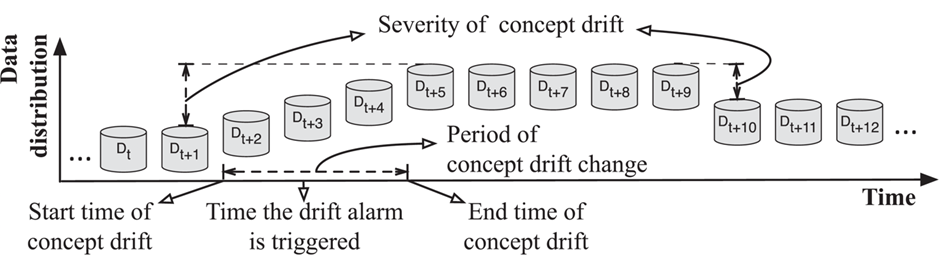
\includegraphics[width=.9\textwidth]{2_Background/figures/concept_drift_understanding.png}
    \caption{Understanding phase of concept drift. \\ \textcolor{gray}{\fontsize{10}{0}\selectfont DOI: 10.1109/TKDE.2018.2876857}}
    \label{fig:concept-drift-understanding}
\end{figure}

%==============================[Adaptation Adaptation]===============
\subsection{Adaptation Phase}
This section delves into strategies for updating existing learning models in response to drift, referred to as drift adaptation or reaction. The three primary categories of drift adaptation methods are simple retraining, ensemble retraining, and model adjusting, each tailored to address specific types of drift.

\begin{enumerate}[label=\Alph*.]
    \item \textbf{Simple Retraining} \\
    One way to respond to concept drift is by retraining a new model with the latest data, replacing the outdated model as shown in Fig.\ref{fig:concept-drift-adaptation}. This approach requires an explicit concept drift detector to determine when to retrain the current model. A window strategy is commonly used, preserving recent data for retraining and/or utilizing old data for distribution change tests. An example of this strategy is Paired Learners \cite{bach2008paired}, which employs two learners: the stable learner and the reactive learner. If the stable learner consistently misclassifies instances correctly classified by the reactive learner, indicating a new concept, the stable learner is replaced with the reactive learner. This method is straightforward, easy to implement, and adaptable at any point in the data stream.
    However, a trade-off arises when adopting a window-based strategy in determining an appropriate window size. A small window better reflects the latest data distribution, while a large window provides more data for training a new model. To address this challenge, the ADWIN algorithm \cite{bifet2007learning} dynamically adjusts sub window sizes based on the rate of change between two sub-windows, eliminating the need for users to predefine window sizes.
    Beyond direct model retraining, researchers have explored integrating the drift detection process with the retraining process for specific machine learning algorithms. DELM \cite{xu2017dynamic}, for instance, extends the traditional ELM algorithm, adapting to concept drift by dynamically adjusting the number of hidden layer nodes in response to increasing classification error rates, indicating a potential concept drift.
    Similarly, FP-ELM \cite{liu2016fp} introduces a forgetting parameter to the ELM model to adapt to drift conditions. A parallel version of the ELM-based method \cite{han2015efficient} has been developed for high-speed classification tasks under concept drift. OS-ELM \cite{soares2016adaptive}, an online learning ensemble of repressor models, integrates ELM using an ordered aggregation (OA) technique to address the challenge of defining the optimal ensemble size.
    In the realm of instance-based lazy learners for handling concept drift, the Just-in-Time adaptive classifier \cite{alippi2008just}  follows the "detect and update model" strategy, extending the traditional CUSUM test \cite{manly2000cumulative} to a pdf-free form for drift detection. When a concept drift is identified, old instances (beyond the last T samples) are removed from the case base. Advancements include extending this algorithm to handle recurrent concepts by considering and comparing the current concept to previously stored concepts \cite{silva2013data} \cite{alippi2008just}. NEFCS \cite{lu2016concept}, another KNN-based adaptive model, employs a competence model-based drift detection algorithm \cite{lu2016concept} to locate drift instances in the case base and distinguish them from noise instances. The redundancy removal algorithm, Stepwise Redundancy Removal (SRR), is developed to eliminate redundant instances uniformly, ensuring that the reduced case base retains sufficient information for future drift detection.
    

\begin{figure}[!ht]
    \centering
    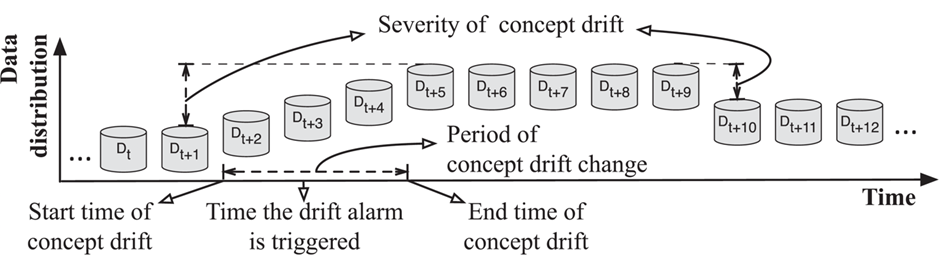
\includegraphics[width=.9\textwidth]{2_Background/figures/concept_drift_understanding.png}
    \caption{Approach for retraining a new model. \\ \textcolor{gray}{\fontsize{10}{0}\selectfont DOI: 10.1109/TKDE.2018.2876857}}
    \label{fig:concept-drift-adaptation}
\end{figure}





\item \textbf{Model Ensemble for Recurring Drift} \\
In recurring concept drift scenarios, preserving and reusing old models can be more efficient than retraining new ones for each recurrence, forming the basis for employing ensemble methods \cite{sun2018concept}. These methods, a focus in stream data mining research, consist of base classifiers with varied types or parameters. Their outputs, determined by specific voting rules, collectively predict new data. Various adaptive ensemble methods, extending classical ones or introducing adaptive voting rules, address the challenges of concept drift as shown in Fig. \ref{fig:concept-drift-ensemble}.
Classical ensemble methods like Bagging, Boosting, and Random Forests have been adapted for streaming data with concept drift. For instance, online Bagging \cite{oza2001experimental} uses each instance once, simulating batch mode bagging. Leveraging Bagging \cite{bifet2009new} employs ADWIN drift detection to replace the existing classifier with the worst performance when concept drift is detected.
 Adaptive boosting \cite{chu2004fast}, monitoring prediction accuracy through a hypothesis test, addresses concept drift, assuming classification errors on non-drifting data follow a Gaussian distribution. The Adaptive Random Forest (ARF) algorithm \cite{gomes2017adaptive} extends the random forest tree algorithm, incorporating concept drift detection (e.g., ADWIN) to decide when to replace an obsolete tree. A similar approach is seen in \cite{li2015learning}, using Beyond classical methods, novel ensemble methods with innovative voting techniques tackle concept drift. Dynamic Weighted Majority (DWM) \cite{kolter2007dynamic} adapts to drifts through weighted voting rules, managing base classifiers based on individual and global ensemble performance. Learn++NSE \cite{elwell2011incremental} addresses frequent classifier additions by weighting them based on prediction error rates.
 Specific types of concept drift are considered in specialized ensemble methods. Accuracy Update Ensemble (AUE2) \cite{brzezinski2013reacting} equally addresses sudden and gradual drift, using a batch mode weighted voting ensemble method. Optimal Weights Adjustment (OWA) \cite{zhang2008categorizing} achieves a similar goal with weighted instances and classifiers. Special cases, like class evolution, are considered in \cite{sun2016online}, while recurring concepts are handled by monitoring concept information \cite{gomes2013mining} \cite{gama2014survey} .Another method \cite{ahmadi2018modeling}, refines the concept pool for recurring concepts.
 
 \begin{figure}[!ht]
    \centering
    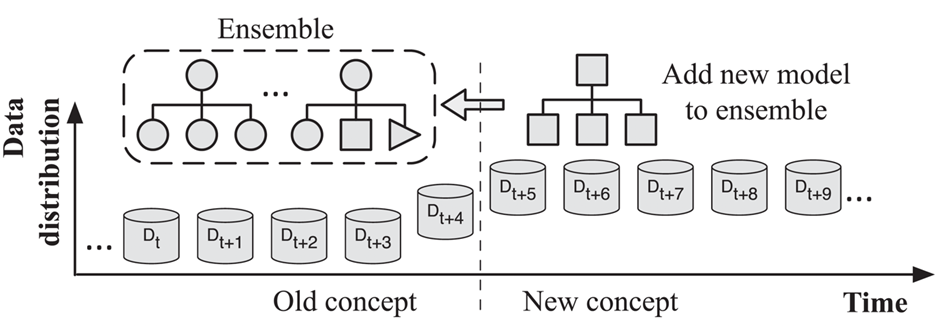
\includegraphics[width=.9\textwidth]{2_Background/figures/ensemble_update.png}
    \caption{Ensemble approach for the adaptation phase. \\ \textcolor{gray}{\fontsize{10}{0}\selectfont DOI: 10.1109/TKDE.2018.2876857}}
    \label{fig:concept-drift-ensemble}
\end{figure}




\item \textbf{Model Ensemble for Recurring Drift} \\
As Shown in Fig. \ref{fig:concept-drift-partial-update}, instead of retraining the entire model, an alternative is to construct a model with adaptive learning capabilities, allowing partial updates in response to changing data distributions \cite{pratama2015evolving}, as in Fig. \ref{fig:concept-drift-partial-update}. This is efficient when concept drift occurs in localized regions. Many techniques in this category use the decision tree algorithm, leveraging its ability to adapt to individual sub-regions.
VFDT \cite{domingos2000mining} is a foundational contribution for high-speed data streams, employing the Hoeffding bound for node splitting. VFDT processes each instance once, doesn't store instances, and has minimal maintenance costs. CVFDT \cite{hulten2001mining}, an extension, addresses concept drift by maintaining a sliding window of the latest data and replacing the original sub-tree with a better-performing alternative.
VFDTc \cite{hulten2001mining} enhances VFDT by handling numerical attributes and adapting to concept drift with node-level detection. Later extensions \cite{yang2012incrementally} \cite{yang2015countering} introduce an adaptive leaf strategy in VFDTc, selecting the best classifier from options like majority voting, Naive Bayes, and Weighted Naive Bayes. Recent studies \cite{rutkowski2012decision}\cite{rutkowski2014new} question VFDT's foundation, the Hoeffding bound, for non-independent variables in information gain. An alternative impurity measure is proposed in a new online decision tree model \cite{rutkowski2014new}, demonstrating its reflection of concept drift and potential use in CVFDT. IADEM-3 \cite{frias2016online} addresses Hoeffding bound concerns by computing the sum of independent random variables for drift detection and pruning.

 \begin{figure}[!ht]
    \centering
    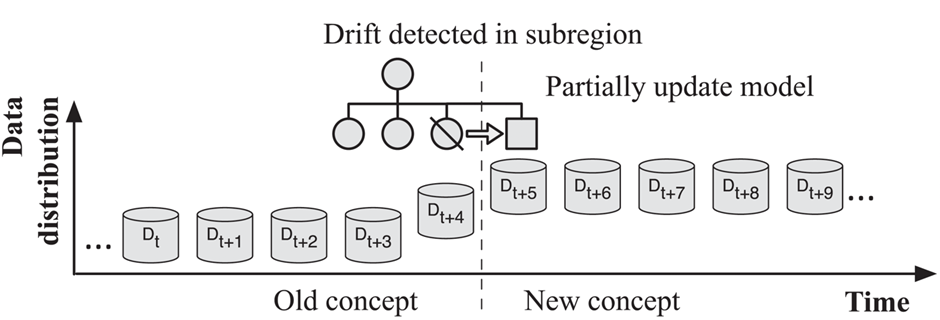
\includegraphics[width=.9\textwidth]{2_Background/figures/partial_update.png}
    \caption{Partial updating approach for the adaptation phase. \\ \textcolor{gray}{\fontsize{10}{0}\selectfont DOI: 10.1109/TKDE.2018.2876857}}
    \label{fig:concept-drift-partial-update}
\end{figure}
\end{enumerate}
% \section{Metrics}
\label{sec:metrics}

The evaluation utilizes several metrics, including recall, precision, F1 score , Balanced Accuracy (BAC), G-mean, and specificity\cite{sasaki2007truth}\cite{kubat1997addressing}\cite{brodersen2010balanced}. These metrics provide a comprehensive view of the classification performance, addressing different aspects such as correctness, balance, and the ability to detect positive and negative cases accurately. The following subsections define each metric used in the evaluation.

\subsection{Recall}
Recall, also known as sensitivity or true positive rate, measures the ability of the classifier to correctly identify positive instances. It is particularly important in scenarios where the detection of positive cases is crucial, such as in medical diagnoses or fraud detection.

\begin{equation}
\text{Recall} = \frac{TP}{TP + FN}
\end{equation}

where $TP$ represents the number of true positives, and $FN$ represents the number of false negatives. A high recall indicates that most of the actual positive cases are correctly classified.

\subsection{Precision}
Precision measures the ability of the classifier to provide relevant positive predictions. It is defined as:

\begin{equation}
\text{Precision} = \frac{TP}{TP + FP}
\end{equation}

where $TP$ represents the number of true positives, and $FP$ represents the number of false positives. Precision is crucial when false positives need to be minimized, for example, in spam detection or quality control systems.

\subsection{F1 Score}
The F1 score is the harmonic mean of precision and recall, and it provides a balanced view of the classifier's performance when both precision and recall are equally important:

\begin{equation}
\text{F1 Score} = 2 \times \frac{\text{Precision} \times \text{Recall}}{\text{Precision} + \text{Recall}}
\end{equation}

A higher F1 score indicates that the model achieves a good trade-off between precision and recall, making it useful in cases where there is an uneven class distribution.

\subsection{Balanced Accuracy (BAC)}
Balanced Accuracy (BAC) is defined as the average of recall for each class, which helps in evaluating the model's ability to correctly classify both positive and negative instances, especially in imbalanced datasets:

\begin{equation}
\text{BAC} = \frac{1}{2} \left( \frac{TP}{TP + FN} + \frac{TN}{TN + FP} \right)
\end{equation}

where $TN$ represents the number of true negatives. BAC is useful when the classes are imbalanced, as it treats both positive and negative classes equally.

\subsection{G-mean}
G-mean is the geometric mean of recall for each class, which measures the balance between classification performance on the positive and negative classes. It is defined as:

\begin{equation}
\text{G-mean} = \sqrt{\frac{TP}{TP + FN} \times \frac{TN}{TN + FP}}
\end{equation}

G-mean is particularly useful in evaluating the performance of models on imbalanced datasets, as it ensures that both classes are predicted with similar accuracy.

\subsection{Specificity}
Specificity, also known as the true negative rate, measures the ability of the classifier to correctly identify negative instances. It is defined as:

\begin{equation}
\text{Specificity} = \frac{TN}{TN + FP}
\end{equation}

where $TN$ represents the number of true negatives, and $FP$ represents the number of false positives. Specificity is crucial in scenarios where false positives need to be minimized, such as in screening tests where a false positive result may lead to unnecessary follow-up procedures.



% state-of-the-art
\chapter{State-of-the-art}
\label{cha:3_State-of-the-art}


In this chapter, we provide a comprehensive review of recent advancements in stream classification, addressing several critical challenges that arise in dynamic data environments. The rapid evolution of data streams introduces complexities such as concept drift, imbalanced multiclass scenarios, class overlap, classifier ensemble selection, emergence of new classes, and the incorporation of transfer learning. This introduction outlines the structure of the chapter and highlights the significance of each topic in advancing stream classification methodologies.
The first section (Setion \ref{sec:3_1_concept_drift}) focuses on concept drift, a phenomenon where the statistical properties of the data change over time. We explore various methodologies developed for real-time detection and adaptation to concept drift in streaming scenarios. This includes a review of techniques that enable systems to identify shifts in data patterns promptly, ensuring sustained classification accuracy. By analyzing the strengths and limitations of these approaches, we highlight the necessity for robust drift detection mechanisms in evolving data streams.
Next, in Section \ref{sec:3_2_ensemble}, we delve into classifier ensemble selection in the context of streaming data. As the characteristics of data streams evolve, selecting the most appropriate ensemble of classifiers becomes crucial. We present algorithms designed to dynamically choose the best-performing classifiers based on the current data distribution. This section emphasizes the importance of adaptive ensemble strategies in enhancing classification performance amidst changing data landscapes.
Section \ref{sec:3_3_imbalanced} addresses the challenges posed by imbalanced multiclass scenarios, particularly in the presence of overlapping classes. We discuss specialized oversampling techniques aimed at countering the effects of class imbalance in streaming data. By providing insights into effective strategies for balancing the representation of minority classes, we lay the groundwork for developing robust frameworks that can maintain performance in imbalanced drifted streams.
As new classes emerge in streaming systems, traditional classifiers often struggle to adapt effectively. In Section \ref{sec:3_4_emergence}, we explore methodologies that specifically focus on the integration of new classes within existing frameworks. This section highlights innovative approaches that enhance the adaptability of stream classification systems, ensuring they remain effective as new data patterns emerge.
In Section \ref{sec:3_5_transfer_learning}, we examine the role of transfer learning in stream classification. This section discusses how transfer learning techniques can leverage knowledge from related tasks to improve classification performance in dynamic environments. We explore current methodologies that facilitate the transfer of information across different domains, particularly in situations where labeled data may be scarce. The insights gained from this discussion will be pivotal for understanding how transfer learning can complement other strategies in our proposed framework.
In Section \ref{sec:3_6_comparsion},To further contextualize our discussion, we conduct a comparative analysis of recent works in the field, focusing on the recent works for each challange. We assess their contributions and identify limitations, illuminating specific gaps in the current research landscape that our work aims to address.
Finally, Section \ref{sec:3_7_remartks} concludes this chapter by identifying key remarks and gaps, which inform the research direction for the subsequent chapters.



%%%%%%%%%%%%%%%%%%%%%%%%%%%%%%%%%%%%%%%%%%%%%%%
%
%   Taxonomies in the Traffic Forecasting Field
%
%%%%%%%%%%%%%%%%%%%%%%%%%%%%%%%%%%%%%%%%%%%%%%%
\section{Concept Drift}
\label{sec:3_1_concept_drift}
Concept drift refers to changes in the underlying data distribution over time, which can reduce the accuracy of previously trained machine learning models \cite{baena2006early, madkour2023historical, tan2022information}. Detecting and responding to concept drift is crucial for maintaining model performance. Several detection methods have been proposed to address this challenge. The Drift Detection Method (DDM) \cite{gama2004learning, bifet2009new} uses a statistical test to identify significant error rate increases, signaling concept drift. The Early Drift Detection Method (EDDM) \cite{gama2004learning, adams2023explainable} extends DDM by considering a moving window of recent data. ADWIN \cite{gama2004learning, adams2023explainable} employs a sliding window to monitor statistical differences and adjusts the window size to adapt to drift patterns. The Kolmogorov-Smirnov windowing method (KSWIN) \cite{adams2023explainable} calculates the Kolmogorov-Smirnov distance to detect drift, while Hoeffding's bounds with moving average test (HDDMA) and its variant HDDMW \cite{gama2004learning, bifet2009new} compute bounds for the true mean to detect distribution changes. Lastly, the Page-Hinkley method \cite{page1954continuous} tracks the cumulative sum of errors, detecting drift when the sum exceeds a threshold. These methods enable machine learning models to adapt to evolving data streams, enhancing model performance and robustness.

%%%%%%%%%%%%%%%%%%%%%%%%%%%%%%%%%%%%%%%%%%%%%%%
%
%   General-purpose Automated Machine Learning
%
%%%%%%%%%%%%%%%%%%%%%%%%%%%%%%%%%%%%%%%%%%%%%%%
\section{Classifier Ensemble Selection}

\label{sec:3_2_ensemble}
This study focuses on the overproduce-and-select approach for classifier ensemble selection methods \cite{cruz2017meta}\cite{kuncheva2000clustering}\cite{jackowski2014improved}. The primary objective of classifier ensemble selection is to identify the optimal subset of classifiers from a larger ensemble, considering various criteria such as performance measures, diversity metrics, meta-learning techniques, and performance estimation approaches. This selection process aims to reduce computational complexity, enhance efficiency, and improve overall ensemble performance, making it highly valuable for real-world applications. By carefully selecting a smaller subset of classifiers, ensemble selection strikes a balance between accuracy and computational resources, adapting to the evolving nature of the data stream. This approach leverages the strengths of different classifiers and adjusts the ensemble composition to handle changing conditions effectively. The goal is to enhance the accuracy, robustness, and overall performance of classification models in dynamic and challenging scenarios. There are two main approaches to the selection process: static and dynamic selection. Static selection assigns classifiers to specific partitions of the feature space, while dynamic selection chooses a classifier specifically for each unknown data sample based on its local competencies. Dynamic Ensemble Selection (DES) is a widely recognized approach that selects the best classifiers for each test instance, considering their competence within the local region of competence. The Randomized Reference Classifier proposed by Woloszynski and Kurzynski \cite{woloszynski2011probabilistic} stands out among various approaches. This classifier introduces randomness through beta distribution, enhancing adaptability and robustness. By considering the stochastic nature of class supports, the Randomized Reference Classifier can potentially improve classification performance in concept drift scenarios. However, it is important to note that employing diversity measures during the classifier selection process, as demonstrated by Lysiak \cite{lysiak2014optimal}, may lead to smaller ensembles but does not necessarily enhance classification accuracy. Overall, the overproduce-and-select approach for classifier ensemble selection methods offers a comprehensive framework for addressing the challenges associated with concept drift. By dynamically adapting the ensemble composition and leveraging the competencies of individual classifiers, this approach aims to improve classification performance, efficiency, and adaptability in dynamic and challenging scenarios.
%%%%%%%%%%%%%%%%%%%%%%%%%%%%%%%%%%%%%%%%%%%%%%%
%
%   Machine Learning for Traffic Forecasting
%
%%%%%%%%%%%%%%%%%%%%%%%%%%%%%%%%%%%%%%%%%%%%%%%
\section{Imbalanced data Streams}
\label{sec:3_3_imbalanced}
In imbalanced data classification, three primary approaches have been identified \cite{yin2022graph}, with our study focusing on the first category that addresses imbalanced data streams through sampling methods, specifically oversampling \cite{ren2023grouping}. This method generates synthetic instances to balance class distributions \cite{nitesh2002smote, han2005borderline, bunkhumpornpat2009safe, maciejewski2011local}. Class imbalance can occur in binary or multi-class scenarios, and our research specifically focuses on multi-class oversampling techniques.

To address multi-class imbalances, Multi-Label SMOTE (MLSMOTE) \cite{charte2015mlsmote} extends SMOTE to multi-class learning by generating synthetic examples for minority class labels and ensuring their proper assignment. A more recent technique, Multi-Label Synthetic Oversampling based on Local Label Imbalance (MLSOL) \cite{yin2022graph}, improves upon MLSMOTE by targeting local imbalances within multi-class classification. MLSOL uses distinct sampling strategies for each label, offering superior performance in classification accuracy and other metrics. It generates synthetic samples from minority class instances in a restricted neighborhood, improving computational efficiency and reducing overfitting, making it a promising technique that outperforms MLSMOTE in several areas.
\section{Streams with Emerging New Classes (SENC)}
\label{sec:3_4_emergence}
Existing methods for detecting new class emergence in streaming data include clustering-based approaches like SACCOS \cite{gao2020saccos}, ECSMiner \cite{masud2010classification}, and SAND \cite{haque2016sand}, which require true labels, limiting their practical use. Similarly, SENC-MaS \cite{mu2017streaming} uses matrix sketches but also needs label information for all instances. Tree-based methods, such as SENCForest \cite{mu2017classification} and SEEN \cite{zhu2020semi}, employ anomaly detection but suffer from high false positives and inefficiencies. SENNE \cite{cai2019nearest} improves detection using nearest neighbor ensembles but lacks model retirement mechanisms, causing longer runtimes. The KNNENS \cite{zhang2022knnens} method combines a k-nearest neighbor ensemble with model updates to address new class detection and classification. However, existing methods generally overlook the use of concept drift techniques, highlighting the need for approaches that can handle both concept drift and new class emergence.

\section{Transfer Learning} 
\label{sec:3_5_transfer_learning}
In recent years, transfer learning has received significant attention due to its growing importance in addressing disparities between source and target domain distributions. Bridging the gap in distribution disparities is vital for optimizing performance in transfer learning, resulting in the development of diverse approaches, which can be broadly categorized into instance re-weighting and feature matching \cite{long2013transfer}. Instance re-weighting methods focus on aligning domain distributions by adjusting the weights of source instances, enabling the reuse of those source instances that closely align with the target domain. Notably, there's a strong emphasis on estimating these instance weights. For example, Huang et al. \cite{long2014transfer} introduced the Kernel Mean Matching (KMM) technique, which calculates weights by minimizing the mean differences between instances from the source and target domains within a Reproducing Kernel Hilbert Space (RKHS). Sugiyama et al. \cite{sun2011two} put forth the Kullback-Leibler Importance Estimation Procedure (KLIEP), utilizing Kullback-Leibler distance as a metric for assessing domain distribution dissimilarity, which includes a model selection step. Building on these instance re-weighting methods, Sun et al. \cite{dai2007boosting} introduced the 2-Stage Weighting Framework for Multisource Domain Adaptation (2SW-MDA) to address challenges in multisource transfer learning. It simultaneously adjusts the weights of source domains and their instances to reduce both marginal and conditional distribution disparities, akin to KMM, while leveraging the smoothness assumption for domain weighting. TrAdaBoost \cite{freund1996experiments}, a variation of the AdaBoost framework \cite{yao2010boosting}, operates by iteratively adjusting the weights of training data. In each iteration, it trains a classifier on a mix of source and target data and uses this classifier to make predictions on the training data. If a source instance is incorrectly predicted, its weight is reduced, diminishing its influence on the classifier. Conversely, the weights of misclassified target instances are increased to amplify their impact. An extension of TrAdaBoost, known as Multisource TrAdaBoost (MsTrAdaBoost) \cite{sun2016return}, is employed to address multisource transfer learning challenges. MsTrAdaBoost combines each source and target dataset, training a separate classifier for each. Subsequently, it selects the classifier with the least error on the target data to update the instance weights.
On a different note, feature matching aims to establish a shared feature representation space between source and target domains, which can be achieved through either symmetric or asymmetric transformations. A typical example of a symmetric transformation is the Transfer Component Analysis (TCA) method by Pan et al. \cite{sun2016return}, employing Maximum Mean Discrepancy (MMD) \cite{zhu2020deep} \cite{long2018transferable}  \cite{long2013transfer} to minimize differences in marginal distribution between source and target domains within an RKHS. Expanding on TCA, Joint Distribution Adaptation (JDA) \cite{wang2020transfer} has been introduced to address both marginal and conditional distribution disparities. Recognizing the varying importance of marginal and conditional distribution differences across different problems, Wang et al. \cite{wang2020transfer} \cite{fernando2013unsupervised} introduced the Balanced Distribution Adaptation (BDA) approach, which introduces a balancing factor. Subspace Alignment (SA) \cite{pearson1901liii} focuses on aligning domain distributions in a lower-dimensional subspace, selecting crucial eigenvectors using principal component analysis \cite{pearson1901liii} and learning a linear transformation matrix to minimize differences in eigenvectors between domains. In contrast, the Distribution Alignment between Two Subspaces (SDA-TS) \cite{pan2010domain} was proposed to align both bases and distributions. Correlation Alignment (CORAL) \cite{rahman2020correlation}, \cite{long2014transfer}, an asymmetric transformation approach, is designed to align sub-space bases and employs second-order statistics. CORAL uses a learned transformation matrix to project source instances into the target domain. While there is a wide range of feature matching techniques in transfer learning, it is imperative to prevent the negative transfer, which occurs when transferred knowledge hinders the performance of target tasks. One of the reasons for negative transfer is the inclusion of unrelated or detrimental source samples in the target domain. To mitigate this, transfer joint matching (TJM) \cite{zhong2009cross} introduces sparsity regularization in the feature transformation matrix, aligning features and re-weighting instances simultaneously. Zhong et al. \cite{cao2018partial} have also developed strategies to mitigate the impact of unrelated source instances and ensure positive transfer. To tackle the challenges posed by partial transfer learning scenarios, where the source domain contains more classes than the target domain, prior works \cite{cao2019learning} \cite{li2020dual} \cite{yang2021concept} introduce instance-level re-weighting and class-level re-weighting mechanisms. These mechanisms are employed to reduce the influence of outlier classes from the source domains. Additionally, another approach presented in \cite{shan2018online} utilizes an adversarial neural network to align domain distributions. In this method, lower weights are assigned to the source samples that are deemed distant from the discriminator. This weighting reflects the perception that such instances have weaker relevance to the target domain. Yang et al. \cite{powers2020evaluation} introduce the HE-CDTL approach for Concept Drift Transfer Learning (CDTL). HE-CDTL leverages knowledge from both source domains and historical time steps within the target domain to improve learning performance. Its key advantages include the utilization of the class-wise weighted ensemble for historical knowledge and the implementation of AW-CORAL for knowledge extraction from source domains. The class-wise weighted ensemble empowers individual classes in the current learning process to select historical knowledge independently. AW-CORAL serves to minimize domain disparities between source and target domains while mitigating negative knowledge transfer. Extensive experiments demonstrate that HE-CDTL outperforms baseline methods in addressing transfer learning challenges in the context of concept drift.
Melanie addresses the challenge of non-stationary environments by considering an online scenario where data in both source and target domains are generated. This method employs an online ensemble to learn models from each domain, subsequently combining these models using a weighted-sum approach. The models are trained incrementally, with their weights dynamically adjusted to handle concept drift. Generally, Melanie can be adapted to address CDTL by substituting the online learning ensemble with an ensemble designed for chunk-based concept drift.

% Define colors
\definecolor{headerColor}{HTML}{4F81BD}
\definecolor{rowColor1}{HTML}{B8CCE4}
\definecolor{rowColor2}{HTML}{DCE6F1}
\definecolor{textColor}{HTML}{000000}
\definecolor{highlightColor}{HTML}{00B0F0}
\section{Comparsion} 
\label{sec:3_6_comparsion}

In this section, we undertake a critical comparison of closely related works addressing the challenges of imbalanced multiclass streams \ref{sec:3_6_1_related_work_imbalanced}, the emergence of new classes \ref{sec:3_6_2_related_work_emergence}, and the integration of transfer learning \ref{sec:3_6_2_related_work_transfer} within streaming environments. The increasing complexity of real-world data streams necessitates advanced methodologies that can effectively manage the intricacies of these challenges. By examining various approaches in the literature, we aim to highlight their contributions, strengths, and limitations in dealing with imbalanced data distributions, adapting to new class occurrences, and leveraging transfer learning techniques. This comparative analysis not only sheds light on the current state of research but also underscores the specific gaps and unresolved issues that our work seeks to address, ultimately paving the way for more robust and adaptive solutions in the realm of streaming data classification.


\subsection{Imbalanced Stream}
\label{sec:3_6_1_related_work_imbalanced}

In the context of multi-class classification, addressing class imbalances is crucial. Multi-Label SMOTE (MLSMOTE) extends the principles of SMOTE to generate synthetic examples for each minority class label, thereby enhancing classifier performance by considering neighboring examples in the feature space. Recently, Multi-Label Synthetic Oversampling based on Local label imbalance (MLSOL) has emerged as a more effective technique. MLSOL systematically addresses local imbalances by employing distinct sampling strategies for each label. Empirical research demonstrates that MLSOL outperforms existing methods, including MLSMOTE, in terms of classification accuracy and computational efficiency. By generating synthetic samples exclusively from minority class instances within a restricted neighborhood, MLSOL produces a more compact and efficient synthetic dataset, mitigating concerns related to overfitting.
As illustrated in Fig. \ref{fig:mlsmote_mlsol}, MLSOL is more likely to select x1 as a seed instance because it is surrounded by more neighbors of the opposite class for l3. MLSMOTE assigns the label vector [0,1,0] to all synthetic instances based on their neighbors. In contrast, MLSOL creates more diverse instances by assigning labels according to their location. Moreover, synthetic instances c2 and c3 generated by MLSMOTE introduce noise, whereas MLSOL copies the labels of the nearest instance to the new examples. In summary, MLSMOTE tends to generate new instances biased toward the dominant class in the local area, whereas MLSOL effectively explores and exploits both the feature and label space.
\begin{figure*}[!ht]

    \begin{center}
      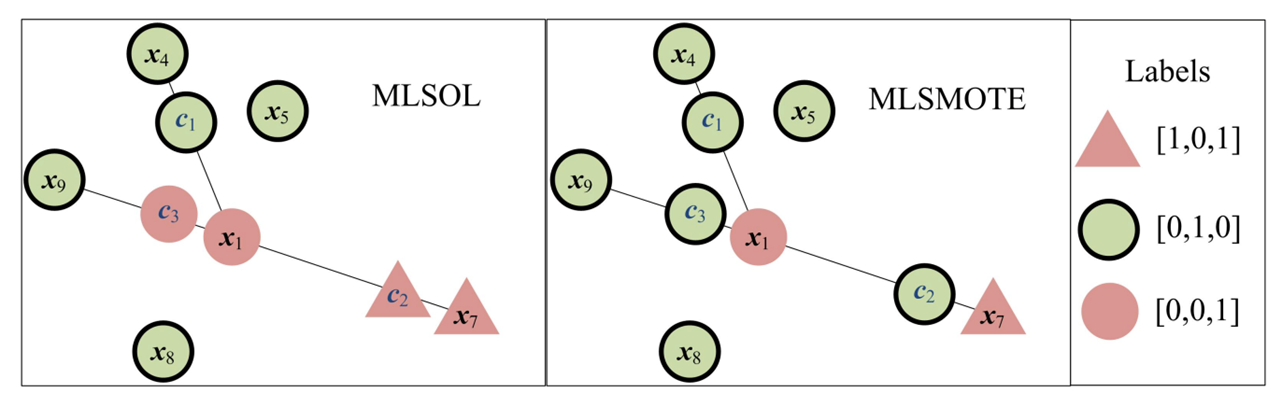
\includegraphics[width=1\textwidth]{3_State-of-the-art/fig/mlsmote_mlsol.png}
    \end{center}

    \caption{Distribution of prediction accuracy. \\ \textcolor{gray}{\fontsize{10}{0}\selectfont DOI: 110.1016/j.patcog.2021.108294}}
    \label{fig:mlsmote_mlsol}

    \end{figure*}
    
Table \ref{table:imbalanced}  presents a comparison of two methods, MLSMOTE and MLSOL, which are designed to address the issue of imbalanced data in multi-class classification. MLSMOTE enhances classifier performance by generating synthetic examples for each minority class label, thereby balancing the class distribution. Its primary advantage is the generation of these synthetic examples, which helps mitigate the imbalance. However, it has significant limitations: the synthetic samples generated might be related to the majority class, which can blur the distinction between classes, and the method struggles with overlapping classes, leading to potential misclassification. On the other hand, MLSOL systematically combats local imbalances by employing distinct sampling strategies for each label within a restricted neighborhood. This localized approach allows MLSOL to generate synthetic examples more precisely, addressing local imbalances effectively. Nonetheless, like MLSMOTE, MLSOL faces challenges with overlapping classes, which can result in misclassification in areas where class boundaries are not clear. Despite its advantages in handling local imbalances, the overlapping class issue remains a critical limitation for both methods, affecting their overall effectiveness in classification tasks.
\begin{table*}[!ht]

    \centering
    \caption{Comparison of the MLSMOTE and MLSOL methods.}
    \label{table:imbalanced}

    \small % Reduce font size
    \renewcommand{\arraystretch}{1} % Reduce cell padding
    \setlength{\tabcolsep}{4pt} % Reduce cell padding
    \setlength{\arrayrulewidth}{0.15mm}

    \begin{tabularx}{\textwidth}{|>{\centering\arraybackslash\bfseries}p{2cm}|
                                       >{\raggedright\arraybackslash}X|
                                       >{\raggedright\arraybackslash}X|
                                       >{\raggedright\arraybackslash}X|}
    \hline
    \textbf{Method} & \textbf{Theory} & \textbf{Advantages} & \textbf{Limitations} \\ 
    \hline
    \textbf{MLSMOTE} & 
    MLSMOTE significantly enhances classifier performance by generating synthetic examples for each minority class label. & 
    Generating synthetic examples for each minority class label. & 
    \begin{itemize}[leftmargin=*]
        \item Random synthetic samples may be related to the majority class.
        \item Overlapping classes.
    \end{itemize} \\ 
    \hline
    \textbf{MLSOL} & 
    MLSOL systematically combats local imbalances within the domain of multi-class classification by employing distinct sampling strategies for each label. & 
    Generating synthetic examples for each minority class label within a restricted neighborhood. & 
    \begin{itemize}[leftmargin=*]
        \item Overlapping classes.
    \end{itemize} \\
    \hline
    \end{tabularx}
    \end{table*}










\subsection{Emergence of new classes}
\label{sec:3_6_2_related_work_emergence}


Effectively detecting and adapting to new classes in streaming data is crucial for maintaining classification accuracy. Tree-based methods like SENCForest and SEEN utilize anomaly detection but face high false positive rates and runtime inefficiencies. SENNE improves detection performance using a nearest neighbor ensemble but suffers from longer runtimes due to the lack of an effective model retirement mechanism. The k-nearest Neighbor Ensemble-based method (KNNENS) addresses new class detection and known class classification using a k-nearest neighbor-based hypersphere ensemble and dynamic model updates. However, a critical limitation of these methods is their inadequate handling of concept drift, which is essential for detecting new classes and retraining the classification model. These methods represent the best closely related work for our proposal, which aims to build upon them by incorporating robust concept drift techniques for more adaptive and resilient classification systems.

Fig. \ref{fig:SENCForest} illustrates the SENCForest approach, which divides the space into three regions (normal, outlying, and anomaly) and detects emerging new classes (anomalies) using a calculated threshold path length. Fig. \ref{fig:SENNE} depicts the SENNE algorithm, where hyperplanes are drawn in three dimensions (x1, x2, and x3) for each class (Fig. \ref{fig:SENNE}a). New instances are then classified as emerging or known classes based on the rank of each class (Fig. \ref{fig:SENNE}b). Fig. \ref{fig:KENNE} presents the KNNENS algorithm, which draws hyperplanes for all class samples (Fig. \ref{fig:KENNE}a), and classifies new instances using a voting mechanism to determine if the instance is an emerging or known class (Fig. \ref{fig:KENNE}b). These visualizations highlight the operational differences between the SENNE and KNNENS algorithms in handling the classification of emerging and known classes.

\begin{figure*}[!ht]
    \centering
    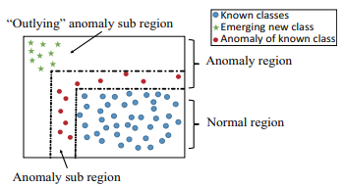
\includegraphics[width=0.85\textwidth]{3_State-of-the-art/fig/SENCForst.png}
    \caption{Overview of stream emerging new classes. \\
    \textcolor{gray}{\fontsize{10}{0}\selectfont DOI: 10.1109/TKDE.2017.2691702}}
    \label{fig:SENCForest}
\end{figure*}
    

\begin{figure*}[!ht]
    \begin{center}
        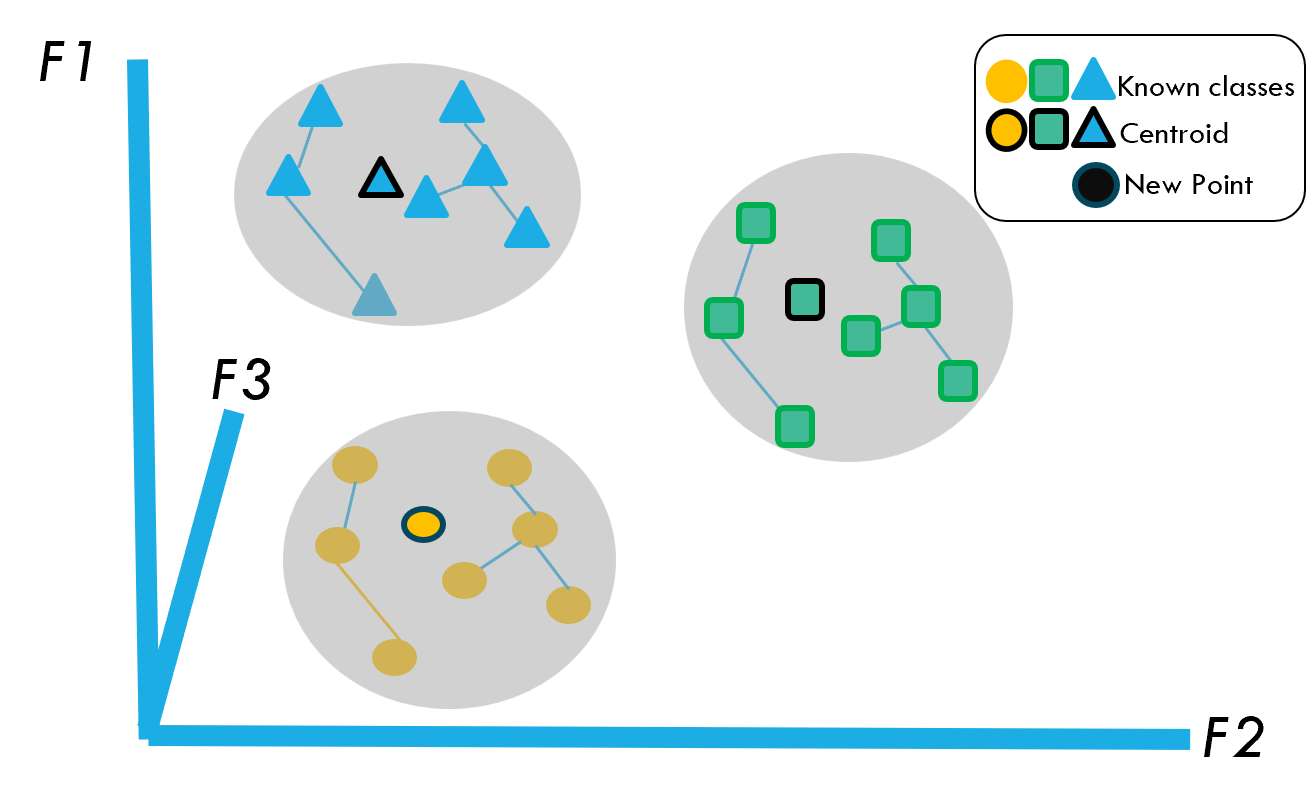
\includegraphics[width=.49\textwidth]{3_State-of-the-art/fig/senne0.png} 
        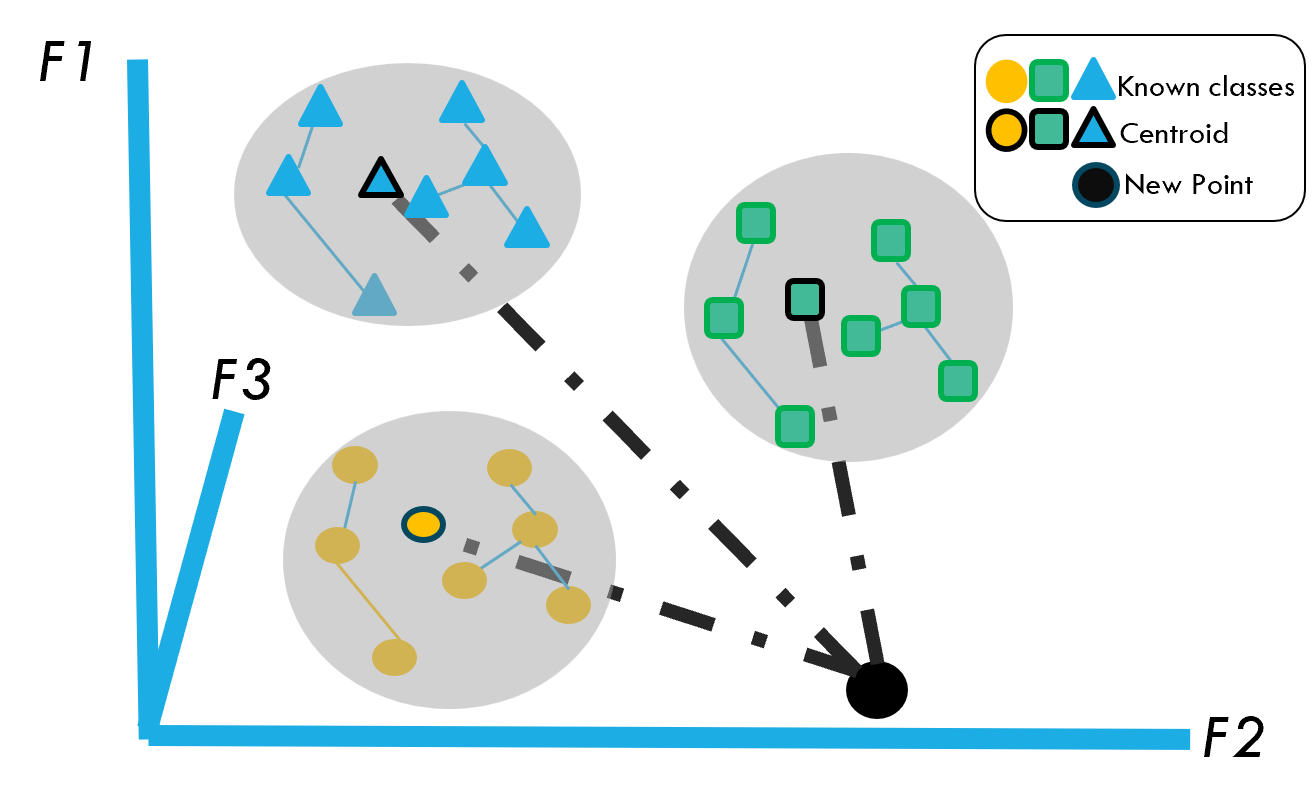
\includegraphics[width=.49\textwidth]{3_State-of-the-art/fig/senne.png} 
        (a)\hspace{6.5cm}(b)
    \end{center}
    \caption{Overview of the Stream Emerging Nearest Neighbor Ensemble (SENNE).}
    \label{fig:SENNE}
    \end{figure*}
    \vline
    \begin{figure*}[!ht]    
        \begin{center}
            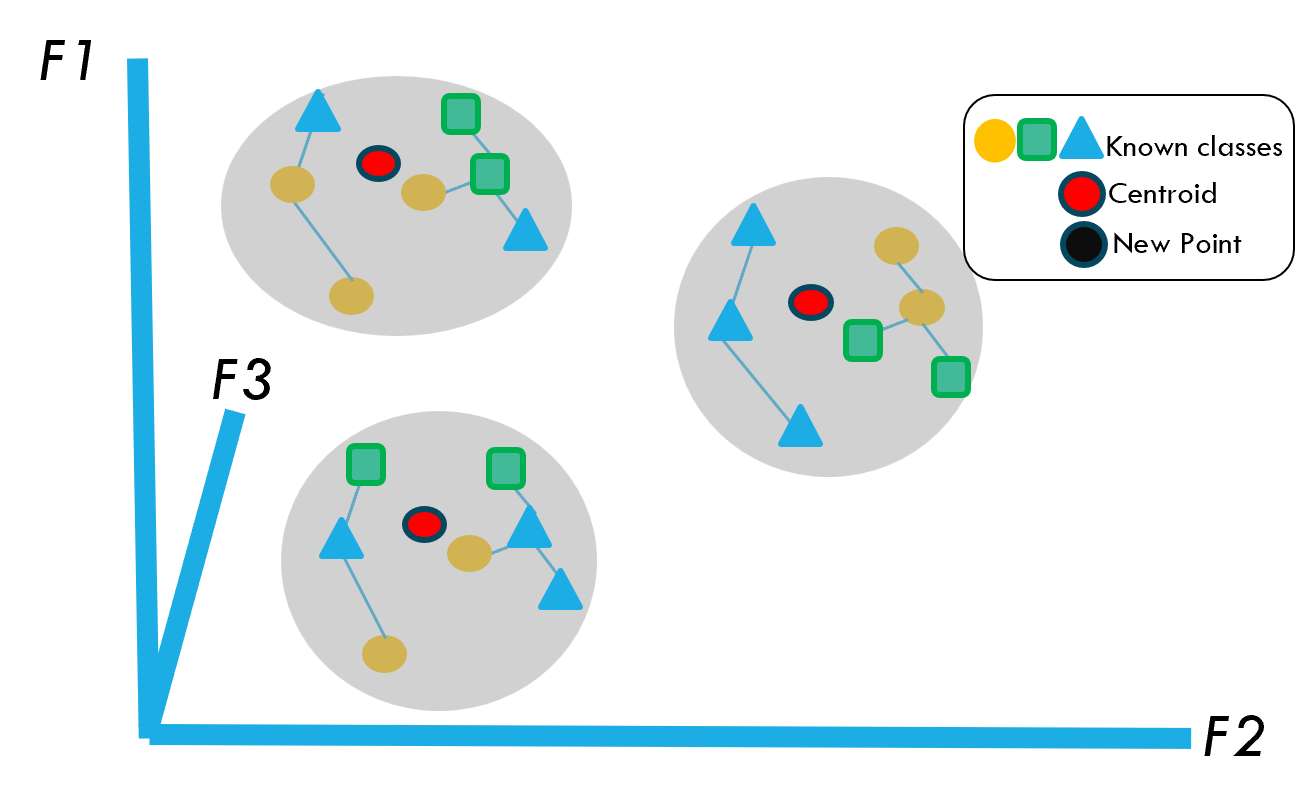
\includegraphics[width=.49\textwidth]{3_State-of-the-art/fig/kenne0.png} 
            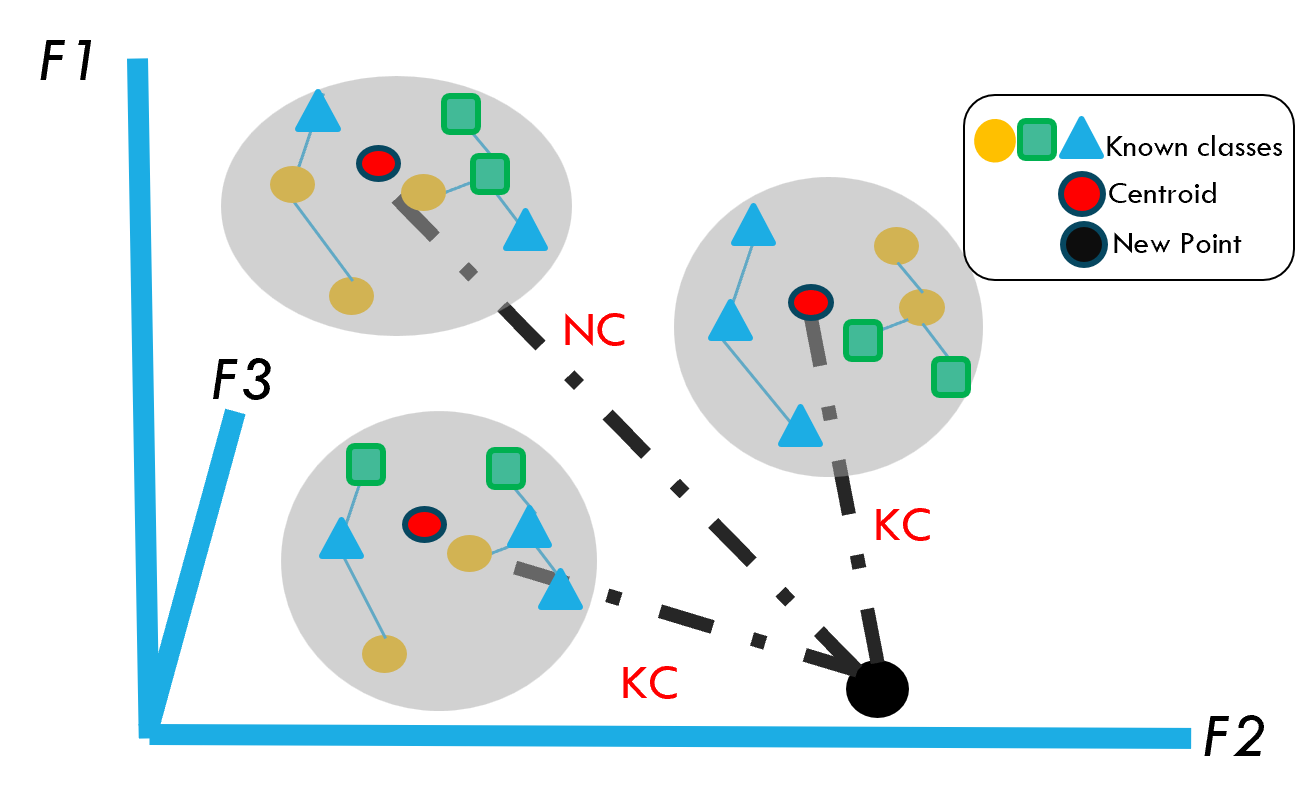
\includegraphics[width=.49\textwidth]{3_State-of-the-art/fig/kenne.png}
            (a)\hspace{6.5cm}(b)
            \end{center}
    
        \caption{Overview of the k-nearest Neighbor Ensemble-based (KENNE).}
        \label{fig:KENNE}
        \end{figure*}
        

        Table\ref{table:emerging} compares three methods for emerging class detection: SENCForest, SENNE, and KNNENS. SENCForest employs the anomaly detection method iForest for new class detection and uses a threshold path to identify anomalies, serving both as an unsupervised anomaly detector and a supervised classifier. However, it has a high potential for false positives and depends on a complex path length threshold. SENNE utilizes a nearest neighbor-based hypersphere of one class ensemble to explore local neighborhood information and sort distances, handling both low and high geometric distances between classes. Its limitations include the assumption that the distribution of known classes remains unchanged and it has lengthy update times. KNNENS employs a nearest neighbor-based hypersphere of all class ensembles to explore local neighborhood information, reducing false positives for new classes without needing true labels for model updates. However, like SENNE, it assumes that the distribution of known classes remains unchanged.

\begin{table*}[!ht]

    \centering
    \caption{Comparison of the SENCForest, SENNE, and KENNE methods.}
    \label{table:emerging}
    \small % Reduce font size
    \renewcommand{\arraystretch}{1} % Reduce cell padding
    \setlength{\tabcolsep}{4pt} % Reduce cell padding
    \setlength{\arrayrulewidth}{0.15mm}
    \begin{tabularx}{\textwidth}{|>{\centering\arraybackslash\bfseries}p{2cm}|
                                       >{\raggedright\arraybackslash}X|
                                       >{\raggedright\arraybackslash}X|
                                       >{\raggedright\arraybackslash}X|}
    \hline
    \textbf{Method} & \textbf{Theory} & \textbf{Advantages} & \textbf{Limitations} \\ 
    \hline
    \textbf{SENCForst} & 
    employs anomaly detection method iForest \cite{wang2010negative} for a new class detection and then applies threshold path to detect the anomalies. & 
    SENCForest serves as both an unsupervised anomaly detector and a supervised classifier.&
    \begin{itemize}[leftmargin=*]
        \item Potential for High False Positives.
        \item Dependency on Path Length Threshold (more complexity).
    \end{itemize} \\ 
    \hline
    \textbf{SENNE} & 
    nearest neighbor-based hypersphere of one class ensemble to explore local neighborhood information and sort distance to calculate distance. & 
    SENNE is able to handle both the low and high geometric distance between two classes in the feature space. & 
    \begin{itemize}[leftmargin=*]
        \item Assumes that the distribution of known classes remains unchanged.
        \item Take long time for update.
    \end{itemize} \\ 
    \hline
    \textbf{KENNE} & 
    nearest neighbor-based hypersphere of all class ensemble to explore local neighborhood information. & 
    KNNENS to reduce false positives for the new class. KNNENS does not require true labels to update the model. & 
    \begin{itemize}[leftmargin=*]
        \item Assumes that the distribution of known classes remains unchanged.
    \end{itemize} \\
    \hline
    \end{tabularx}
    \end{table*}













\subsection{Transfer Learning}
\label{sec:3_6_2_related_work_transfer}

In the realm of transfer learning, three prominent methods—CORAL, Melanie, and HE-CDTL—serve as closely related approaches to our proposed method. Correlation Alignment (CORAL) is an asymmetric transformation approach that aligns sub-space bases using second-order statistics. By employing a learned transformation matrix, CORAL projects source instances into the target domain, thereby minimizing domain discrepancies and reducing negative knowledge transfer. Melanie addresses the challenge of non-stationary environments through an online ensemble learning approach. It incrementally trains models from both source and target domains, dynamically adjusting their weights to handle concept drift, and combines these models via a weighted-sum approach as shown in Fig. \ref{coral_fig}. As Shown in Fig. \ref{cdtl_fig} This method can be extended to Concept Drift Transfer Learning (CDTL) by using an ensemble for chunk-based concept drift. HE-CDTL, designed explicitly for CDTL, leverages knowledge from source domains and historical time steps within the target domain to enhance learning performance. It utilizes a class-wise weighted ensemble for historical knowledge and implements AW-CORAL for extracting knowledge from source domains. The class-wise weighted ensemble allows individual classes to select historical knowledge independently, while AW-CORAL minimizes domain disparities and mitigates negative knowledge transfer. Extensive experiments have shown HE-CDTL to outperform baseline methods in addressing transfer learning challenges in the context of concept drift. Together, these methods provide a comprehensive framework for effective transfer learning in dynamic and evolving data environments.

Table\ref{table:transfer} compares three methods: CORAL, Melanie, and HE-CDTL. CORAL (Correlation Alignment) utilizes a learned transformation matrix and Singular Value Decomposition (SVD) to project source instances into the target domain, effectively minimizing domain discrepancy and reducing negative knowledge transfer. However, it faces challenges with non-stationary and heterogeneous data. Melanie (Multisource Online Transfer learning for Non-stationary Environments) addresses online learning problems where data in source and target domains are generated from non-stationary environments. Its advantages include considering online problems but it too is limited by the complexities of online learning and data heterogeneity. HE-CDTL (Class-wise Weighted and Domain-wise Ensemble) minimizes domain shift by aligning second-order statistics of source and target distributions, leveraging historical knowledge to reduce disparities between domains. Despite its strengths, it relies on the quality of the source domain and also struggles with heterogeneous data.
\begin{figure*}[!ht]

    \begin{center}
        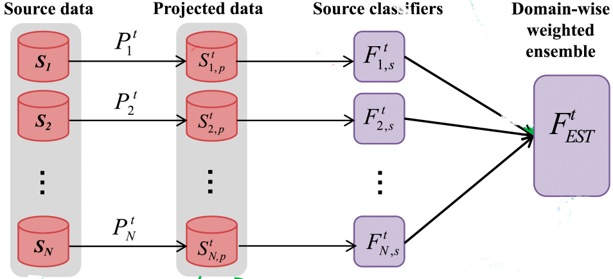
\includegraphics[width=.85\textwidth]{3_State-of-the-art/fig/coral.png} 
    \end{center}
    \caption{Overview of CORrelation ALignment (CORAL)}
    \label{coral_fig}
    \end{figure*}
    \begin{figure*}[!ht]    
        \begin{center}
            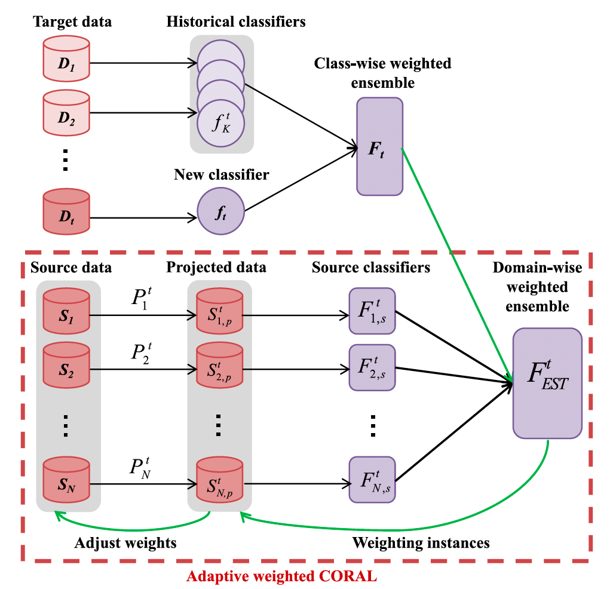
\includegraphics[width=.85\textwidth]{3_State-of-the-art/fig/cdtl.png} 
        \end{center}
        \caption{Overview of Concept Drift Transfer Learning (CDTL).}
        \label{cdtl_fig}

        \end{figure*}

\begin{table*}[!ht]
    \centering
    \caption{Comparison of the CORAL, Malanie, and CDTL methods.}
    \label{table:transfer}
    \small % Reduce font size
    \renewcommand{\arraystretch}{1} % Reduce cell padding
    \setlength{\tabcolsep}{4pt} % Reduce cell padding
    \setlength{\arrayrulewidth}{0.15mm}
    \begin{tabularx}{\textwidth}{|>{\centering\arraybackslash\bfseries}p{2cm}|
                                       >{\raggedright\arraybackslash}X|
                                       >{\raggedright\arraybackslash}X|
                                       >{\raggedright\arraybackslash}X|}
    \hline
    \textbf{Method} & \textbf{Theory} & \textbf{Advantages} & \textbf{Challenges} \\ 
    \hline
    \textbf{CORAL} & 
    Correlation Alignment (CORAL) uses a learned transformation matrix and Singular Value Decomposition (SVD)  to project the source instances into the target domain. & 
    CORAL can minimize domain discrepancy across
source and target domains, meanwhile reducing the negative
knowledge transfer. & 
    \begin{itemize}[leftmargin=*]
        \item Non-stationary environments.
        \item Heterogenous multisource.
    \end{itemize} \\ 
    \hline
    \textbf{Melanie} & 
    Multi-sourcE onLine TrAnsfer
learning for Non-statIonary Environments (Melanie). utilize the class-wise weighted . & 
It considers
an online problem in which the data in source and target
domains are generated from non-stationary environments. & 
    \begin{itemize}[leftmargin=*]
        \item Online Learning based only.
        \item Heterogenous multisource.
    \end{itemize} \\
    \hline
    \textbf{MLSOL} & 
    HE-CDTL uses the class-wise weighted and domain wise ensemble for historical knowledge and reduce the disparities between the source and target domains . & 
    HE-CDTL minimizes domain shift by aligning the second-order statistics of source and target distributions. & 
    \begin{itemize}[leftmargin=*]
        \item Depend on Source Domain Quality.
        \item Heterogenous multisource.
    \end{itemize} \\
    \hline
    \end{tabularx}
    \end{table*}

\section{Remarks} 
\label{sec:3_7_remartks}

By comparing the literature on ensemble learning for classification tasks, the proposals in this thesis differ from other studies in several ways:

\begin{enumerate}
    
    \item [-] As evident from our literature review on imbalanced streams, most studies have concentrated on generating synthetic samples while ignoring class overlap. \textit{To address this challenge}, we propose an approach to generate non-overlapping classes in imbalanced streams.

    \item [-] Oversampling techniques often perform inefficiently in the presence of concept drift. \textit{To tackle this issue}, we introduce a methodology that selects the oversampling technique based on the current and historical distribution of the stream chunks.
    
    \item [-] Our literature review on non-stationary environments reveals that most works focus on detecting emerging new classes while overlooking distribution changes. \textit{To overcome this challenge}, we propose a combined approach utilizing Dynamic Ensemble Selection (DES) to select the best classifier for each chunk based on stream distribution, k-means clustering, and concept drift to address both emerging new class detection and distribution changes.
    
    \item [-] In our literature review on transfer learning, we observed that most studies focus on homogeneous multisource transfer and neglect heterogeneous multisources in non-stationary environments. \textit{To resolve this issue}, we propose a combined approach integrating Dynamic Ensemble Selection (DES), Concept Drift Transfer Learning (CDTL), eigenvector techniques, and concept drift to address heterogeneous transfer learning in non-stationary environments.

\end{enumerate}



% the back matter: appendix and references close the thesis
\backmatter
\include{0_frontmatter/summary-arabic}


%: ----------------------- appendix ------------------------

%\appendix


%: ----------------------- bibliography ------------------------



% The section below defines how references are listed and formatted
% The default below is 2 columns, small font, complete author names.
% Entries are also linked back to the page number in the text and to external URL if provided in the BibTex file.


% Original version:

% PhDbiblio-url2 = names small caps, title bold & hyperlinked, link to page
%\begin{multicols}{2} % \begin{multicols}{ # columns}[ header text][ space]
%\begin{tiny} % tiny(5) < scriptsize(7) < footnotesize(8) < small (9)
%
%\bibliographystyle{Latex/Classes/PhDbiblio-url2} % Title is link if provided
%\renewcommand{\bibname}{References} % changes the header; default: Bibliography
%
%\bibliography{9_backmatter/references} % adjust this to fit your BibTex file
%
%\end{tiny}
%\end{multicols}



% Show all bibliography entries
%\nocite*

% If we want bibliography backreference, use unsrt first and the desidered one after

%\bibliographystyle{unsrt} % Defines the bibliography style

%\bibliographystyle{alpha} % Defines the bibliography style

\bibliographystyle{Latex/StyleBST/IEEEtran} % Defines the bibliography style

%\bibliographystyle{apa-good} % Defines the bibliography style
%\bibliographystyle{natbib} % Defines the bibliography style

%\bibliographystyle{plainurl}

%\renewcommand{\bibname}{References} % changes the header; default: Bibliography

%To include the references/works cited/bibliography in your Table of Contents, right before the bibliography command, use the command
%\addcontentsline{toc}{section}{References}
%

\bibliography{11_backmatter/references} % adjust this to fit your BibTex file

% --------------------------------------------------------------
% Various bibliography styles exit. Replace above style as desired.

% in-text refs: (1) (1; 2)
% ref list: alphabetical; author(s) in small caps; initials last name; page(s)
%\bibliographystyle{Latex/Classes/PhDbiblio-case} % title forced lower case
%\bibliographystyle{Latex/Classes/PhDbiblio-bold} % title as in bibtex but bold
%\bibliographystyle{Latex/Classes/PhDbiblio-url} % bold + www link if provided

%\bibliographystyle{Latex/Classes/jmb} % calls style file jmb.bst
% in-text refs: author (year) without brackets
% ref list: alphabetical; author(s) in normal font; last name, initials; page(s)

%\bibliographystyle{plainnat} % calls style file plainnat.bst
% in-text refs: author (year) without brackets
% (this works with package natbib)


% --------------------------------------------------------------


%: Declaration of originality
%\include{9_backmatter/declaration}





\end{document}
